\documentclass[syuuron]{kuee}
\usepackage[dvipdfmx]{graphicx}
\usepackage{kueecite}
\usepackage{amsmath}

\title{評価構造における単語間の関係性可視化に関する研究}
\author{小澤 啓太}
\professor{小山田 耕二 教授}
\course{京都大学大学院 工学研究科}
\department{電気工学専攻}
\date{平成28年2月4日}

%%% 本文
\begin{document}
\maketitle
\tableofcontents


%%%序論
\chapter{序論}
	%%%人々の評価基準を解明するって大事!
	人の持つ評価基準を理解することは,多くの人にとって重要である.
	企業では,商品を開発する際に他商品よりも高く評価してもらう商品を開発することが求められる.
	現在,多くの企業にとって市場は自国だけでなく世界全体へと移行しつつあり,
	消費者の好みは年齢や性別,経済力だけでなく国,宗教などによって多様化している.
	そのため,人々がどんな点を評価するのかという評価基準と評価基準の因果関係の詳細な調査が必要であり,
	多くの企業では市場調査や商品購入者からの評価が行われている.
	
	%%%人々の評価を解明する評価グリッド法とは?
	人々の評価基準や評価基準の因果関係を解明する手法の一つに評価グリッド法という,半構造化インタビューを用いた定性調査手法がある.
	評価グリッド法では,人間がある対象物を知覚して,その知覚からどのように理解し,どのように評価するのかを明らかにすることができ,
	環境心理学やマーケティング調査,感性工学といった分野で日本を中心に幅広く利用されている\cite{sen1}.
	評価構造は「良い,悪い」など,評価的判断に寄与している理解の単位 (評価項目) と,評価項目の間に存在する因果関係から構成され,
	ネットワーク図として表現されることがある(図~\ref{fig:es1}).
	ネットワーク図で表現する場合,図~\ref{fig:es2}のようにノードは評価項目を表しており,文章でラベル付けされている.
	また,評価項目間の因果関係をネットワーク図のエッジで表現する.
	マーケティング分野などでは,評価構造を分析することで,人間の評価基準や評価基準の因果関係を把握でき,
	人間の求める商品の推測につながるので,評価構造の効果的な分析方法に関する要求が高まっている\cite{egm6}\cite{egm7}.
	それに伴い,評価構造の分析に関する研究は数多く行われている~\cite{egm8}\cite{egm9}.
	従来の評価構造は,模造紙や付箋などに手書きすることで作成される場合が多く,多人数の評価構造を作成,分析するのに多くの時間を要した.
	しかし,近年ではE-Grid\footnote{http://egrid.jp}のような,評価グリッド法によるインタビューや評価構造分析をサポートするWebアプリケーションも開発され,
	評価構造作成及び分析の効率化が進んでいる~\cite{egm6}\cite{egm10}.
	
	%%%従来での問題
	E-Gridのような評価グリッド法を支援するアプリケーションが増加し評価構造作成の効率化が進む一方で,問題も発生している.
	それは,評価構造の大規模化に伴う視認性の低下,それによる評価構造分析の非効率化である.
	従来の手書きでの作成では多人数の評価構造を統合することが困難であったが,Webアプリケーションなどの登場により容易に行えるようになった.
	多人数の評価構造が統合されることで,評価項目とエッジ数が増加し,
	指定された領域内で評価構造全体を表示するには評価構造のレイアウトサイズを縮小する必要があった. 
	縮小された評価構造では,図~\ref{fig:es3}のように評価項目の文字や評価項目間の関係性が見づらくなり,分析することが困難である.
	評価構造を分析する際の着目点として,評価構造内での頻出語の発見や頻出語と因果関係を持つ項目の把握があげられる.
	評価構造内で頻出する単語とは,多くの人が回答した内容であり,多くの人が共有する評価項目である.
	また,頻出語と隣接する評価項目を知ることで,多くの人が共有する評価項目の因果関係を知ることができる.
	このように,頻出する評価項目や頻出語と隣接する評価項目を発見することで消費者の評価構造を把握することができるが,
	縮小されたネットワーク図では頻出語や評価項目間の関係性が見えづらく,分析を短時間で行うことが困難である.
	従来の評価構造分析手法では,評価構造を構成する評価項目間の因果関係に着目して因果関係の定量化を行う手法は数多く提案されている~\cite{egm8}\cite{egm9}.
	しかし,評価構造の分析手法の多くはネットワーク図表示をもとにした分析である.
	ネットワーク図では上記のような見やすさに関する問題があるので,ネットワーク図以外での表示を行う必要がある.
	
	テキストデータの概観にはWord Cloudというテキストデータ可視化手法が有効である.
	Word Cloudとは,文章中で出現頻度が高い単語を複数選び出し,その頻度に応じた大きさで図示する可視化技術である\cite{wc1}.
	評価構造をWord Cloudで可視化する場合は評価構造のテキストを単語で区切り,
	単語の出現頻度にもとづき単語のフォントサイズを決定することで,テキストデータ内の重要語を可視化することができる.
	しかし,Word Cloudではテキストデータを形態素や単語などに区切ることで,評価項目間の関係性など
	文として持っていた情報を切り離してしまうという問題があげられる.
	この問題を解決するためには,評価項目間の関係性など文として持っていた情報を同時に可視化することが求められる.
	
	%%%提案手法!手法の説明,実験の要約
	以上の問題を解決するために本論文は,評価項目内に出現する単語の頻度と,
	評価構造内での単語間の位置関係を反映した評価構造データ向けのテキストベースの可視化手法を提案した.
	提案手法では,評価構造内の評価項目の文章を形態素解析し,その結果抽出した単語をWord Cloudで可視化する.
	Word Cloudとは文章中で出現頻度が高い単語を複数選び出し,その頻度に応じた大きさで図示する可視化技術である.
	また,提案手法ではWord Cloud内の単語の配置座標を,本論文で提案する評価構造内単語の座標計算手法を適用し決定した.
	提案する評価構造内単語の座標計算手法では,はじめに評価構造内での各単語間の位置関係をネットワーク図の最短距離を用いて計算する.
	この単語の位置関係を多次元尺度構成法により二次元の値に縮小し,この値をWord Cloud内での単語の配置座標とする.
	これにより,単語間の距離から因果関係を持つ項目の発見が容易になった.
	しかし,単語の配置座標決定時は単語間の重複が発生し,単語間の関係が分かりづらくなる可能性があるので,
	単語間の位置関係を維持しつつ重複阻止を行った座標を再計算しWord Cloud内の単語の配置座標と決定する.
	重複阻止では単語間の相対的位置関係の保持を行いつつ,指定領域の最大活用するためのフォントサイズの最適化も行う.
	これにより,単語数に応じて最適なフォントサイズ,評価構造内での単語の位置関係を保持した読みやすい可視化を達成した.
	Word Cloudによる可視化は似た内容の評価項目の統合にもつながり,規模の大きい評価構造の場合でも分析を行いやすくなる.
	しかし,提案手法による可視化結果は一部の情報を可視化することに有効だが,インタラクションを加えなければ評価構造分析が困難であった.
	そこで,評価構造のネットワーク図と提案手法による可視化結果を併置したシステムを提案し,
	インタラクションを加えることでより効率的な分析を可能とする.

	%%%提案手法のもたらす効果
	本論文では,評価構造のWord Cloud可視化の有効性,Word Cloud内の単語配置方法の有効性を検証するために二種類の比較実験を行った.
	一つは,評価構造のWord Cloud可視化の有効性を測るために比較実験である. 
	評価構造のネットワーク図とWord Cloud可視化による比較実験を行い,
	単語数が多い場合の評価構造の頻出単語の発見,頻出語と因果関係を持つ単語の発見に関してWord Cloud可視化が有効であることを証明した.
	もう一つは,Word Cloud内の単語配置方法の有効性を検証するため,
	単語をランダムに配置した場合と提案手法に基づき配置位置を決定した場合とでの比較実験を行った.
	比較実験により,頻出単語の発見が容易になり,単語の座標関係から頻出語と因果関係の強い単語の把握に有効であることが証明された.
	また,提案システムの評価としてシステムを利用した評価構造の分析を行ってもらい,その後にシステムに関するユーザーにアンケートを行った.
	この結果から,提案システムは多くの人の共有する評価基準や,その因果関係の分析が用意になったことが確認された.

	%%%論文構成
	本論文の構成は以下の通りである.
	第1章は,本論文の序論である.第2章は,本論文の関連する研究について述べる.第3章では,提案手法と使用するデータの説明を行う.
	第4章では,開発した提案システムについての詳細を述べる.
	第5章では,提案手法,提案システムを用いた評価実験の内容を述べる.
	第6章では第5章で行った評価実験の結果を,第7章では,評価実験をもとにした考察を行う.
	最後に,第8章では本論文の結論と今後の課題について述べる.

		\begin{figure}
			\begin{center}
				\fbox{
				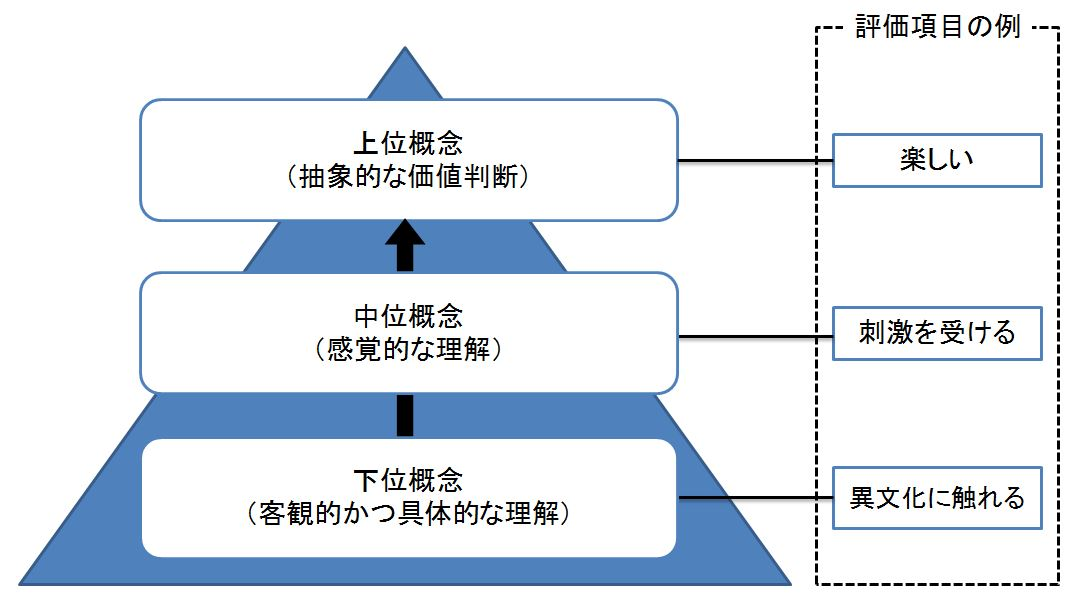
\includegraphics[width=\linewidth]{./png/es1.JPG}
				}
			\end{center}
			\caption{評価構造の構成}
	  		\label{fig:es1}
		\end{figure}
		\begin{figure}
			\begin{center}
				\fbox{
				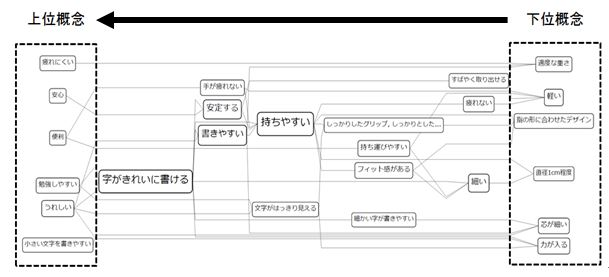
\includegraphics[width=\linewidth]{./png/es2.JPG}
				}
			\end{center}
			\caption{評価構造1}
	  		\label{fig:es2}
		\end{figure}
		\begin{figure}
			\begin{center}
				\fbox{
				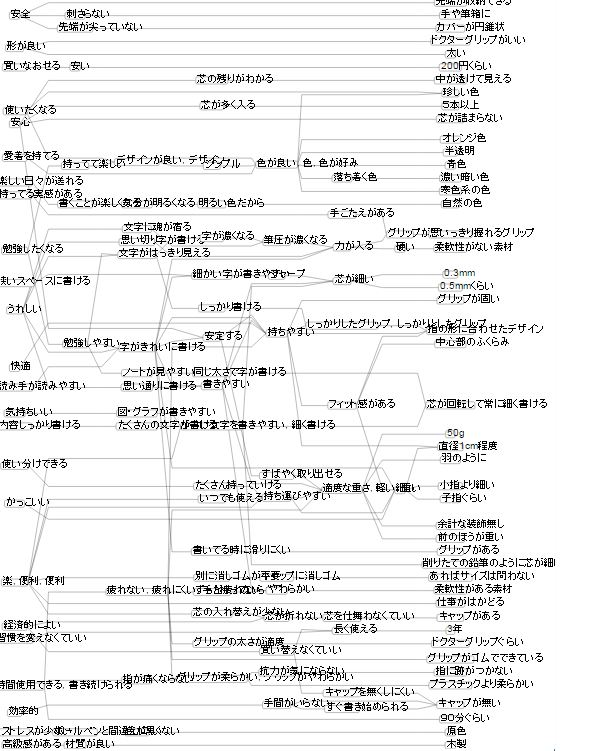
\includegraphics[width=\linewidth]{./png/es3.JPG}
				}
			\end{center}
			\caption{評価構造2}
	  		\label{fig:es3}
		\end{figure}

%%%関連研究
\chapter{関連研究}
	本研究は,評価構造の文章の頻出語や関係性の可視化に関するものである.本章では,評価構造を可視化する評価グリッド法に関する研究,
	テキストデータ内の頻出語や関係性の可視化に関する研究,評価構造をWord Cloudで可視化する際に使用する単語の重複阻止法に関する研究に分けて関連研究を述べる.
	\section{評価構造と評価グリッド法}
		%%%評価グリッド法のインタビュー手法内での立ち位置
		評価グリッド法とは,市場調査を行うために行われる定性調査手法の一つである.
		市場調査で行われる手法にはアンケート調査やエスノグラフィック・アプローチなど様々ある.
		その中で評価グリッド法は,質問の流れがある程度決まっている半構造化インタビュー手法なので,
		エスノグラフィック・アプローチのような観察手法や非構造化インタビュー手法と違い,客観性・説得性を確保しやすく,
		アンケート調査のような構造化インタビューと違い,指定された内容以外の回答を得ることができる.
		また,評価グリッド法は,基本的に回答者とインタビュアーによる1対1の面談式インタビューを行われるので,
		個人の深層心理を聞くことが可能である.
		%%エスノグラフィック・アプローチ参考文献
		
		%%%評価グリッド法の誕生話
		評価グリッド法は讃井らが提案したインタビュー手法であり,Kellyらが提案したレパートリー・グリッド法\cite{rg1}
		という認知構造抽出手法を改善した手法であることから,提案当初はレパートリー・グリッド発展法という名称でもあった.
		讃井らは,ラダーリング法\cite{rd1}を取り入れることで,認知構造のうち評価に関与する部分のみを抽出することを可能にした.
		ラダーリング法は「〇〇だと何故良いのか,〇〇のどういうところが好きなのか」という質問を繰り返す手法である.
		評価グリッド法では評価に関与する部分のみを選択的に抽出することでインタビュー時間の削減を行った.
		
		%%%評価グリッド法の目的,適用先
		讃井らは,住居設計の際に居住者の住環境評価のプロセスを把握することの重要さから,評価グリッド法を開発した.
		評価グリッド法は開発当初,住宅や環境関する評価調査に適用されており,
		高橋らは年代,性別,教育環境別の美しいと思えるインテリア空間の傾向を確かめた\cite{egm1}.
		また,近年では商品企画にも適用分野を広げており,商品企画の際に役立つ手法である商品企画七つ道具の一部として幅広く利用されている\cite{egm2}.
		
		%%%評価グリッド法の行い方
		評価グリッド法はまずテーマ設定を行う.
		何についての評価構造を作成するか決定し,比較対象を準備する.
		評価グリッド法では,比較対象のことを刺激要素と呼び,
		インタビューを行うにあたって,複数個の刺激要素を準備しておく.
		例として,欲しいシャープペンシルについての評価構造を作成する場合,
		複数個のシャープペンシルもしくはその写真を用意する必要がある.
		準備が終わった後にインタビューが開始される.
		インタビューは図~\ref{fig:egm1}で表すようにオリジナル評価項目の抽出とラダーリングの繰り返しである.
		オリジナル評価項目は刺激要素の比較から抽出される.
		オリジナル評価項目の抽出では,はじめに刺激要素を比較し順序付けを行う.
		その後に,順位が隣り合う刺激要素を2つずつ取り上げ,回答者にどちらの刺激要素のほうが好ましい,もしくは好ましくないかを選択させる.
		選択させた後に,質問者は回答者に選択した要素のほうが好ましい,もしくは好ましくないと思った理由を尋ねる.
		この回答をオリジナル評価項目として記録し,回答をオリジナル評価項目としてグラフに描く.
		理由が複数個ある場合は,それらを全てオリジナル評価項目として記録し,グラフに描く.
		ラダーリングではこのオリジナル評価項目を起点としてインタビューを行う.
		ラダーリングでは,オリジナル項目の上位概念及び下位概念の抽出を行う.
		上位概念とはより抽象的な価値判断を表し,下位概念はより客観的かつ具体的な理解のことを表す.
		上位概念を抽出する方法をラダーアップと呼び,
		オリジナル評価項目としてあげられた理由「○○」について,「〇〇だと何故いいのですか」と質問を行い,回答された理由を上位概念として記録する.
		また,下位概念を抽出する方法をラダーダウンと呼び,
		オリジナル評価項目としてあげられた理由「△△」について,「具体的にどういうところが△△なのですか」と質問を行い,回答された理由を下位概念として記録する.
		ラダーアップでは,回答された上位概念についてラダーアップを行い,それ以上の上位概念が引き出せなく成るまで続け,
		ラダーダウンでも同様にそれ以上の下位概念が引き出せなく成るまで繰り返す.
		途中で理由が複数個挙げられた場合は,上位概念及び下位概念を枝分かれさせつつ同様の手順を繰り返す.
		ラダーリングで抽出したオリジナル評価項目の上位項目と下位項目はグラフにマッピングする.
		刺激要素全てのペアに対してオリジナル評価項目の抽出とラダーリングを行えばインタビューを終了する.
		以上の手法を取ることにより,評価構造はある概念に対する評価を明らかにすることができるとされている.
		
		%%%評価構造と評価グリッド法の関係
		評価グリッド法によって作成されたネットワーク図を評価構造と呼ぶ(図~\ref{fig:es2}).
		評価構造は,評価グリッド法から取得した評価項目と評価項目間の因果関係をネットワーク図で表現している.
		評価グリッド法のインタビューは基本的には回答者と質問者の2人で行い,個人毎の評価構造を作成する.
		商品企画などでは複数人の評価構造を統合した全体評価構造を作成し分析を行う.
		評価構造は,調査対象者の評価基準を概観することや,
		多くの人が共有する評価理由,予想外の評価理由の発見などに有効である.
		
		%%%評価構造に関する研究
		讃井らは人々の住環境に関する評価構造を作成し,個人が持つ住環境評価の実態を明らかにした.
		また,評価グリッド法では個人毎の評価構造を統合し全体の評価構造を作成する場合もある.
		その際,評価構造内の評価項目間の因果関係について分析するために評価項目間の因果関係を定量化する分析手法が数多く提案された.
		尾上らは,満足度の高い学会についての因果関係を調べるため,評価項目間の因果関係モデルの構築を行った\cite{egm8}.
		評価グリッド法での結果からアンケート項目を設計及び実施し,アンケート結果をもとにグラフィカル連鎖モデリングを用いた因果関係モデルの構築と構造方程式モデリングによる分析を行った.
		他にも,アンケート結果をもとに重回帰分析やパス解析,階層分析,共分散構造分析などを行う研究も提案されている.
		本村らは,評価グリッド法により抽出したスケルトン構造を基にしてベイジアンネットの統計的学習により定量的なモデルを構築し,確率推論アルゴリズムの適用を行った\cite{egm9}.
		
		%%%評価構造の新たな問題と自分の研究の立ち位置の説明
		評価グリッド法は,従来は紙ベースで実施されることが多く,分析作業などにおいて調査者の負担が大きかった.
		しかし,近年は評価グリッド法のインタビューと分析を支援するソフトウェアも開発され,多人数の評価構造の統合が容易になった.
		土田らが開発した評価グリッド法支援ツールEGM-assistは代表例の1つである\cite{egm11}.
		また,商品企画七つ道具の支援ソフトウェアであるPLANPARTERは評価グリッド法を支援している\cite{egm12}.
		以上のような評価グリッド法支援ソフトウェアは評価グリッド法に基づいたインタビューの効率化する.
		また,尾上はE-Gridという評価構造を分析するソフトウェアを提案している.
		以上のように評価構造の作成や統合が容易になることにより評価構造内のノード数が増え,評価構造の概観や分析が困難になった.
		評価構造を分析する場合ノードのラベルを読む必要があるが,限られた領域に表示する必要があるので,
		ノード数が増加するとノードの表示領域が小さくなり,ラベルの視認性が低下してしまう.
		この問題に対して尾上らは評価項目数の削減を行った\cite{net1}.
		各評価項目のネットワーク中心性を計算し,ネットワーク中心性の低い各評価項目を表示しないことで,問題を解決した.
		本論文は,二つの方法から問題解決を行った.
		一つ目の方法は助詞や助動詞などの意味無し語を排除.二つ目の方法は評価構造内で複数回出現する単語の出現回数を一度に減少させることで,
		重要度が低いが意味を持つ単語の領域を確保しつつ,従来より視認性の高い評価構造の可視化に成功した.
		
	\section{テキストデータ分析}
		%%%テキストデータ分析の概要と例
		本研究では前節で述べたように,評価構造が持つテキストデータを分析することで,
		頻出単語の発見,頻出語と強い関係を持つ単語の発見することを目的としている. 
		テキストデータ分析は共起分析やテキスト要約など様々な目的のもと行われており,
		KH Coderのような,テキストデータを統計的に分析するためのフリーソフトウェアも開発されている.
		KH Coderとは下位頻出語を確認するリスト表示や語と語の結びつきを調べる共起ネットワーク表示,
		似た内容の文書をまとめるクラスター分析などで様々な観点から分析を行うことができる.
		
		%%%テキストデータ分析の歴史
		KH Coderのようなコンピュータを用いたテキストデータ分析は古くから数多く提案されてきた.
		1960年台の後半には,既に2つのテキスト分析アプローチが提案されていた.
		一つはDictionary-basedアプローチと呼ばれ,分析者が分類基準を作成し,
		分析者の持つ理論や問題意識を操作化するためのアプローチである\cite{kh3}.
		Dictionary-basedアプローチはコーディング規則を設けることで,データを絞り,様々な側面からデータを見ることができるという利点である.
		その反面,意図的に理論や仮説に都合の良いコーディングが作成される危険も存在する.
		もう一つは,Correlationalアプローチと呼ばれるもので,分析者の理論仮説や問題意識により汚染されていない状態で,
		多変量解析などによってコンピュータにデータ分析してもらうアプローチである.
		近年では,この二つのアプローチを統合したアプローチが提案されている\cite{kh1}\cite{kh2}.
		はじめにCorrelationalアプローチによりデータ全体を要約し,
		その結果を元にコーディングを作成しDictionary-based アプローチを用いる手順を踏むことで,
		分析者の持つ理論や問題意識の影響を極力受けない形でデータを分析することが可能となる.
		提案手法も同様に二つのアプローチからテキスト分析を行う.
		
		%%%テキストデータ分析の順序
		Dictionary-basedアプローチに関する研究は数多く行われている.
		テキスト内で頻出する特徴語を抽出することや,語と語の関係性を調査するために階層クラスター分析や共起ネットワークを行う手法,
		内容が似た文書の群を探すクラスター分析など多岐にわたる.
		提案手法では,前章で述べたように評価構造内の頻出語や単語間の関係性の分析を行うための可視化を行うことを目的としている.
		そこで提案手法では,はじめにDictionary-basedアプローチとして評価構造内の頻出語や単語間の関係性を可視化し,
		次にCorrelationalアプローチとして選択した単語の共起語の強調表示などを行った.
		
		%%%単語間の関係性分析の例
		テキストデータ内の単語の関係性の可視化に関して,ネットワーク可視化や多次元尺度構成法などが挙げられる.
		ネットワーク可視化の例としては,単語にノード, 
		そして共起した単語間にエッジを定義する共起ネットワークなどがあげられる.
		その他にも,keyword-in-context検索結果をネットワーク可視化する手法は数多く提案されている.
		WattenbergらはWordTreeを提案した\cite{wt1}.
		WordTreeでは検索結果がツリー構造上で可視化され,可視化結果を対話的に操作することで効率的に文章を探索することができる.
		Riehmannらも,keyword-in-context検索結果を可視化する例文検索ツールWORDGRAPHを提案した\cite{wg1}.
		WORDGRAPHもWordTreeと同様に検索結果をツリー構造上で可視化するが,
		各例文で共起する単語が存在する場合に,共起単語の部分で合流させることで例文をまとめ視認性を向上させた.
		また,WORDGRAPHではワイルドカードを含むkeyword-in-context検索結果を可能としていた.		
		多次元尺度構成法では,高次元属性を持つ分類対象物を低次元空間における点の布置で表現する手法であり,
		Word Cloudで可視化する際に単語間の距離で関係性を表すことに利用される\cite{wc2}.
		ErickらはWeb検索結果の可視化を次元削減を用いて行った\cite{or1}.
		検索結果のページのテキストデータからそれぞれ文書ベクトルを生成し,次元削減を行うことで文書ベクトルが近い検索ページが近くに配置される.
		同時に,クラスタリングを行うことで,検索結果に複数分野の情報がある場合に目的の分野の情報を発見しやすくなった.
		また,多次元尺度構成法によって求めた座標をWord Cloudで可視化する研究も提案されている.
		Word Cloud可視化の一例としてWordleがあげられる\footnote{http://www.wordle.net/}.
		WordleはJonathanによって開発されたWord Cloudを作成するWebベースのツールであり,
		新聞のようなマスメディアや教育分野など幅広く利用されている\cite{wc2}.
		単語のフォントサイズや色,単語をランダムに配置するレイアウトによってユーザーの想像力をひきたて,新しい知見を生みやすくする.
		また,Word Cloudでは単語の座標から単語間の関係性を可視化することが可能である.
		Adaらは,アメリカ合衆国の三人の大統領就任演説の比較を行うために,
		演説で読まれたテキストをWord Cloudで可視化した\cite{fta2}.
		単語のフォントサイズはtfidf値から計算し,単語間のコサイン類似度から単語の座標を決定した.
		また,コサイン類似度から計算した単語座標では,単語が重複する可能性があったので,
		Xiaodiらが提案したForce Transfer algorithm(FTA)を用いて重複の阻止を行った\cite{fta1}.
		提案手法ではWord Cloud内の単語座標を,Wordleのようなランダム配置ではなく,
		Adaらのような単語座標を単語間のコサイン類似度ではなく,単語間のネットワーク図内での距離関係から決定した.
		これは,本研究の目的である評価項目間の関係性の可視化を行うためである.
		そのため,本研究ではグラフ構造を持つ評価構造のテキストデータから単語間の関係性を可視化するために,
		評価構造内のテキスト間距離を考慮して,テキストに含まれる単語間の距離行列を作成し,
		多次元尺度構成法を用いることで単語の座標を決定することで,
		単語間の位置関係から評価構造内での単語の関係性を読み取れるようにした.
		ネットワーク図では,ノード数が増加する場合にエッジ数も同様に増加するので,全てのノードとエッジを表示すると視認性が低下する可能性が高くなる.
		これに対して,Word Cloud による可視化では,意味無し語の削減だけでなく,似た内容の評価項目の統合が可能となり,
		エッジ表示を行わないことで,規模の大きい評価構造の場合でも,視認性が低下せず,分析が行いやすくなるものと期待できる.
		また,提案手法を用いたシステムではユーザーが単語を選択すると選択単語が出現する評価項目の上位概念,
		下位概念の単語との関係をリアルタイム表示する機能を新たに開発することで単語の関係性を読み取れるようにした.
		以上のように,Word Cloudを用いて必要最低限の情報のみを可視化することで,単語の関係性の情報を残しつつ視認性が低下することを防いだ.
		
	\section{重複阻止}
		%%%重複阻止の概要
		前節では,テキストベースの可視化の一つとして,単語の位置座標を計算したWord Cloudによる可視化について触れた.
		提案手法のように,単語の属性が多次元データで定義される場合,これを次元削減し二次元データに変換する.
		この二次元データ基づき,その単語を平面に配置する際,他の単語との間に重複が存在しないようにすることが望ましい.
		このような重複問題は,ネットワーク図でも問題とされており,重複阻止手法は古くから研究がされている.
		重複阻止に関する研究では,以下の美的基準のいずれかを考慮したレイアウトを生成されている\cite{fta2}\cite{or2}.
		\begin{itemize}
			\item 対象の相対的位置関係を保持する
			\item 対象間の距離関係を維持する
			\item 指定された領域からはみ出さない
			\item 指定領域の空白部分を減らす
		\end{itemize}
		
		%%%重複阻止その1(fta論文参考)
		重複阻止手法では大きく三種類のアプローチが提案されていた.
		一つ目は,均等スケーリングである.均等スケーリングでは,図形やオブジェクトを全ての方向に同じ倍率で拡大または縮小するアプローチである\cite{fsa1}.
		このアプローチでは,オブジェクトの相対的位置関係や距離関係は維持されるものの,図形やオブジェクトを不必要に移動させる必要があり,
		指定領域を大幅に拡大する必要が出てくるという問題が発生する.
		
		%%%重複阻止その2
		二つ目のアプローチは,力学モデルである.
		力学モデルでは,グラフを対象としており,グラフのノードとエッジに仮想的な力を割り当て,力学的エネルギーの低い安定状態を探すことで重複を阻止する.
		XiaodiらはFTAを提案した\cite{fta1}.
		FTAでは一定の規則に基づきオブジェクトを選択し,重複オブジェクトが存在するか調べる.
		重複オブジェクトを発見した場合,重複オブジェクトを水平方向か垂直方向かに移動させる力を発生させる.
		移動する方向は重複が解除されるまでに移動する距離が短い方向を選択する.移動したオブジェクトと重複する他のオブジェクトも同距離同方向に移動する.
		移動が終わったら他のオブジェクトを探し,同様の操作を行う.以上の操作を繰り返す手法である.
		FTAでは,対象間の距離関係を維持した重複阻止が達成された.
		StrobeltらはRwordle-Cを提案した\cite{rwc1}.
		Rwordle-CはFTAと同様に一定の規則に基づきノードを選択し,重複ノードの有無を調べ,
		重複ノードを発見した場合,重複ノードを渦状に移動させる.初期位置を渦の中心とし広がるように移動させ,重複が解除される位置まで移動させる.
		力学モデルを用いた重複阻止では,均等スケーリングに比べ,レイアウトがコンパクトになる利点があるが,
		上記の力学モデルをWord Cloudに適用すると,単語の文字列の方向と重複阻止のために移動する方向の相関が強く,
		指定領域をはみ出すことや,指定領域内に空白部分が多く残るという問題が発生する.
		
		%%%重複阻止その3
		三つ目のアプローチは,この問題を解決するために提案されたもので,条件付き最適化を適用する.
		条件付き最適化では,重複問題を制約条件のある最適化計算に置き換えることで重複を阻止する.
		Erickらは,可視化対象の座標を変数とした目的関数を作成し座標を計算する手法を提案した\cite{or1}.
		NEIGHBORHOOD PRESERVING SNIPPET LAYOUTでは,目的関数に重複阻止と単語の距離関係の維持を目的とした関数を作成することで
		対象間の距離関係を保持しつつ.重複の発生しない座標計算を可能とした.
		また,Erickらは目的関数に,制約条件を追加した最適化手法も提案している\cite{or2}. 
		可視化対象は二次元空間に配置されている点群であり,はじめに指定領域内で格子を生成し,格子内で座標点が存在する四角(セル)だけを残し,
		セルのx,y座標,セルの辺長を変数として最適化する.
		最適化計算を行う際に,相対的位置関係保持,セル間の重複阻止,指定領域の最大利用,指定領域外へのセルのはみ出し禁止など,
		複数の制約条件を設けることで適切なセル配置を可能にした.
		このように,条件付き最適化では複数の美的基準を制約条件に置き換えることで様々な条件を満たした重複阻止を可能とする.
		提案手法ではErickらが提案したエネルギー関数を用いた重複阻止の最適化計算手法を参考にし,
		Word Cloudで表示する単語内の1文字を格子の1セルと置き換え,セルの位置の最適化計算を行った.
		また,Erickらの制約条件を一部修正し新制約条件を追加することでWord Cloudでの単語配置に適した座標計算を可能とした.
		
		\begin{figure}
			\begin{center}
				\fbox{
				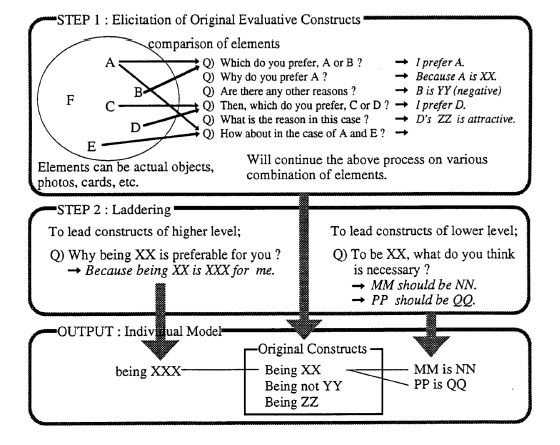
\includegraphics[width=\linewidth]{./png/egm1.JPG}
				}
			\end{center}
			\caption{評価グリッド法の手順\cite{egm6}}
	  		\label{fig:egm1}
		\end{figure}

%%%本提案システム
\chapter{提案手法}
	本章では,提案手法である,評価構造のテキストデータから単語のWord Cloud内座標を計算するまでのプロセスと使用する評価構造のテキストデータの説明を行う.
	
	\section{使用データ}
		この節では,提案手法で使用する評価構造データについて説明する.
		提案手法では,評価項目のラベルであるテキストと評価項目の回答者数,評価項目間の隣接リストを使用する.
		評価項目のラベルであるテキストから形態素解析を行い,形態素に分割する.
		この形態素をWord Cloudで可視化する単語として使用する.
		評価項目の回答者数と評価項目間の隣接リストは,単語間の距離行列を計算する際に使用する.
		
		本研究では,E-Gridを用いて評価構造データの作成を行った.
		E-Gridとは,評価グリッド法に基づいた評価構造の抽出や分析をビジュアル的に支援するシステムであり,
		評価構造を抽出する機能から評価構造データを作成した.
		E-Gridでのインタビューは1人ずつで行い,個人の評価構造を作成した.
		その後,回答者全体の評価構造を把握するため,個人毎の評価構造を統合し全体の評価構造を作成した.
		E-Gridにより作成される評価構造データは評価項目と隣接する評価項目,評価項目の回答者数 ,評価項目のテキストラベル,評価項目の回答者名等の情報を記載されている.
		提案手法では,形態素解析に日本語形態素解析システムMeCab\cite{mcb1}と形態素解析辞書Unidicを使用した.
		Unidicは,語彙素・語形・書字形・発音形の階層構造を持つので,表記の揺れや語形の変異にかかわらず同一の単語と識別することが可能である.
		提案手法では,表記の揺れや語形の変異がある単語はそれぞれの単語の語彙素を表示する.
		以上から得られたデータに以下のプロセスを通し可視化を行う.		
		
	\section{座標計算}
		提案システムでの可視化プロセスは図~\ref{fig:met1}のように大きく3つに分けられる.
		はじめに,評価構造データから評価構造内単語間の距離行列を作成する.
		次に,評価構造内単語間の距離関係を保持したまま単語をWord Cloud可視化するため,次元削減法を用いて各単語のx,y座標を計算する.
		計算した座標では単語間の重複が発生する場合があるので,
		単語の重複を排除し,しかし単語間の位置関係を崩さず,指定領域を最大限活かすことのできる単語の座標を再計算する.
		Word Cloudに可視化する際は再計算された座標を使用する.
		以下の項では,可視化プロセスの詳細を説明する.
		
		\subsection{単語間距離行列の作成}
			前章で記述したとおり,提案手法ではWord Cloud内の単語の座標を評価構造内での単語の距離関係を考慮して決定する.
			評価構造内単語間の距離関係は単語が使用されているノードの距離関係から計算され,単語間距離行列Dで表す.
			単語間距離行列Dは,評価構造から計算される出現行列F,ノード間距離行列U,重み行列A から計算される.
			図~\ref{fig:met2}は評価構造と評価構造から取得された出現行列F,ノード間距離行列U,重み行列Aの例を表す.
			以下ではノード間距離行列U,出現行列F,重み行列Aの導出方法を述べる.
			$ノード群はN \in \bigl\{n_{1},n_{2},...,n_{l} \bigl\},単語群はW \in \bigl\{w_{1},w_{2},...,w_{m} \bigl\},で表す.$
			$またノードn_iを回答した人数をa_i,単語w_iの全ノードでの使用回数をu_iと表す.$
			
			\subsubsection{ノード間距離行列}
				ノード間距離行列Uは,各ノード間の距離関係を表す行列である.
				ネットワーク図のノードViとVjの最短距離の経路でノードをn個経由する場合,
				第i行第j列と第j行第i列の要素がn+1となる行列である.
				また,対角成分の値は全て0である.
				最短経路の計算は幅優先探索アルゴリズムを使用した.
				本研究では,MATLABを用いて幅優先探索を行った\cite{int1}.
				このアルゴリズムは横型探索とも言われ,以下のルールに従って探索を行う.
				
				\begin{enumerate}
					\item 根ノードを空のキューに加える.
					\item ノードをキューの先頭から取り出し,以下の処理を行う.
						\begin{itemize}
							\item ノードが探索対象であれば,探索をやめ,結果を返す.
							\item そうでない場合,ノードの子で未探索のものを全てキューに追加する.
						\end{itemize}
					\item もしキューが空ならば,グラフ内の全てのノードに対して処理が行われたので,探索をやめ"not found"と結果を返す.
					\item 2に戻る.
				\end{enumerate}
				
				\begin{eqnarray}
				 U = \left(
				    \begin{array}{cccc}
				    	u_{11} & \ldots & u_{1l} \\
				    	\vdots & \ddots & \vdots \\
				    	u_{l1} & \ldots & u_{ll}
					\end{array}
				 \right)
				\end{eqnarray}	
		
			\subsubsection{出現行列}
				出現行列Fはノードと単語の関係を表す行列である.
				出現行列の列は評価構造内のノードを,行は全ノードから形態素解析を行い取り出した全ての単語群を表す.
				i行目の単語がj列目のノードの文章に出現しない場合は0となる.
				出現する場合,i行目の単語がn個のノードで使用されていると第i行第j列の要素は1/nとなる.
				要素の値を使用回数の逆数とすることで単語が複数のノードで出現する際に単語間距離を平均の距離となる.
				この行列から各ノードに出現する単語を知ることができる.
				\begin{equation}
				 	F = \left(
				    \begin{array}{cccc}
				    	f_{11} & \ldots & f_{1l} \\
				    	\vdots & \ddots & \vdots \\
				    	f_{m1} & \ldots & f_{ml},\\ 
					\end{array}
					\right),
				 	f_{ij} = \left\{ \begin{array}{ll}
						\frac{1}{u_i} & (n_i \in w_j) \\
				    	0 & (otherwise)
				  	\end{array} 
				  	\right.
				\end{equation}
				
			\subsubsection{重み行列}
				各ノードの重み行列Aは,各ノードの回答者数を表す行列である.
				対角成分以外の値は全て0とし,対角成分は回答者数の逆数とする.
				i番目のノードの回答者数がnの場合,第i行第i列の要素は1/nとなる.
				提案手法では,頻出語の関係性をより詳細に可視化するため,頻出語ほど距離行列の値が小さくなるよう設定した.
				\begin{equation}
				 A = \left(
				    \begin{array}{cccc}
				    	a_{11} & \ldots & a_{1l} \\
				    	\vdots & \ddots & \vdots \\
				    	a_{l1} & \ldots & a_{ll} \\
					\end{array}
				 \right),
				 a_{ij} = \left\{ \begin{array}{ll}
				     0 & (i ≠ j) \\
				     \frac{1}{a_i} & (i = j)
				  \end{array} \right.
				\end{equation}

				
				
			上記の式(3.1),(3.2),(3.3)によって行列F,U,Aを計算した後,
			以下の式(3.4)によって単語間距離行列Dを計算する.
			$ネットワーク図内の単語w_iとw_jの最短距離の平均値が,$
			第i行第j列と第j行第i列の値となる行列である.
			\begin{eqnarray}
			 D = \frac{1}{2} FAUA^{\mathrm{T}}F^{\mathrm{T}}
			   = \left(
			    \begin{array}{cccc}
			    	d_{11} & \ldots & d_{1m} \\
			    	\vdots & \ddots & \vdots \\
			    	d_{m1} & \ldots & d_{mm}
				\end{array}
			 \right)
			\end{eqnarray}	
			
		\subsection{次元削減}
			次に,評価構造内単語間の距離関係を保持したまま単語をWord Cloud可視化するため,単語のx,y軸の値を求めるために次元削減を行う.
			次元削減を行うことで,各単語に2次元の値を与え,この2次元の値を単語のx,y軸の値にする.
			提案システムでは多次元尺度構成法を適用することで次元削減を行う.
			多次元尺度構成法とは,多変量解析の一手法である. 分類対象物の関係を低次元空間における点の布置で表現する.
			多次元尺度構成法では,始めにヤング・ハウスホルダー変換を施す.
			ヤング・ハウスホルダー変換は距離の2乗の行列に両側から中心化行列をかける演算であり,以下の式で表す.
			\begin{eqnarray}
				P = - \frac{1}{2} JDJ^{\mathrm{T}}
			\end{eqnarray}
			$単語数をnとすると,行列Jは単位行列から全要素に1/nの行列を引いたn \times n行列を引いたn \times n行列$
			$行列Dは点 x_i と x_j の間の距離 d_{ij} の2乗を要素とするn \times n行列である.$
			次に,Pをスペクトル分解することで固有値,固有ベクトルを求め,固有値の大きい方から2つ取り,対応する固有ベクトルを取り出す.
			各単語のx, y座標は取り出した2つの固有ベクトルの値となる.
			
		\subsection{重複阻止}
			最後に,計算した座標では単語間の重複が発生するので,単語間の相対的位置関係を崩さないように単語の重なりの除去を行う.
			提案手法ではErickらが提案した重複阻止手法を参考にした\cite{or2}.
			Erickらの提案手法では指定領域内にセルと呼ばれる正方形の図形が配置されており,
			セルの重心座標を最適化計算する手法である.
			Erickらの手法では,セル間の相対的位置関係保持,セル間の重複阻止,指定領域の最大利用を達成する最適なセルの座標を計算する.
			提案手法では単語内の1文字を1セルと置き換え,各単語はセルが水平方向に隣接する長方形となる.
			そのため,最適化計算をする座標はセルと呼ばれる正方形の重心座標ではなく,
			セルが隣接する長方形の重心座標と変更した.
			以下の節では最適化計算で用いる目的関数,制約条件の説明を行う.
			
			指定領域に配置する単語の集合を$G= \bigl\{g_1,g_2,…,g_n \bigl\}$とし,
			単語の各文字すなわち各セルの集合を$H= \bigl\{h_{11},h_{12},…,h_{1p},h_{21},…,h_{nq} \bigl\}$とする.
			各単語は,$g_{i}=(x_{i},y_{i},w_{i})$で表される.
			$(x_{i},y_{i})$は単語 $g_{i}$ の重心点,$w_{i}>0$ は辺の縦の長さである.
			$w_{i}$ は$w_{ij} = \alpha_i \delta $と表し,
			$ \alpha_i $は単語 $g_{i}$ の最頻出語との辺の縦の長さの比であり $ \alpha_i=  e_i⁄(max⁡(e_1,e_2,…,e_n))$ , 
			$ \delta_i $は最適化後の最頻出語の辺の長さであり $ \delta_i= max⁡(w_1,w_2,…,w_n)$ と表す.
			$e_i $ は単語 $ g_i $ の評価構造内での出現頻度を表す.
			各セルは縦,横の辺の長さが $W \times H$である指定領域内でセル間の大きさの比率を維持しつつ,
			セル間の重複阻止と指定領域の最大利用,セル間の相対的位置関係の保持を達成するように再編成される.
			図~\ref{fig:met3}は$x_{ij},y_{ij}$と$ \delta $,$W,H$の例である.
			
			\subsubsection{重複阻止問題}
				指定領域内で単語を再編成するために,提案手法では単語の再編成を以下のように最適化問題として定式化した.
				
				\begin{equation}
					\begin{aligned}
					& \text{minimize}   && \sl{E(\bf{z})} = \sl{E_{comp}(\bf{z})} + \sl{E_{resize}(\bf{z})} \\
					& \text{subject to} && A \bf{z} \le \bf{b},  \bf{z} = [\bf{x}^T \: \bf{y}^T \: \bf{r}^T \: \bf{\delta}]^T,\\
					&                   && \bf{x} = (x_1,x_2,...,x_N)^T \in \bf{R}^N \\
					&                   && \bf{y} = (y_1,y_2,...,y_N)^T \in \bf{R}^N \\
					&                   && \bf{r} = (r_{12},...,r_{1N},r_{23},...,r_{2N},...,r_{N−1N})^T,
					&                   && \bf{r_{ij}} \in {0,1} \\
					&                   && \delta \le min(W,H).
					\end{aligned}
				\end{equation}
								
				$\bf{z} は求める変数である$.
				$ \bf{x},\bf{y} はセルの重心座標$, $ \bf{r} は単語の重複を防ぐための調整変数,\delta は再編成後の最頻出語の辺の長さを表す変数である$.
				$A,\bf{b} は最適化問題の制約条件を表す行列である$.
				$エネルギー項 \sl{E_{comp}(\bf{z})}, \sl{E_{resize}(\bf{z})} はそれぞれ単語と指定領域を操作する関数である$.
				前者は単語間重複と相対的位置関係の保持を考慮する単語集約エネルギー項,後者は指定領域を可能な限り最大利用するための指定領域最大利用エネルギー項である.
				以下では2つのエネルギー項についての詳細を述べる.
			
				\paragraph{単語集約エネルギー項}
					一つ目のエネルギー関数 $\sl{E_{comp}(\bf{z})} $ は単語集約エネルギー項であり,
					この関数の目的はセルを狭い範囲で簡潔に表すことである.
					エネルギー関数$ \sl{E_{comp}(\bf{z})} $は,セルの重心座標を変数とした二次間数で以下の式で表す.
					\begin{equation}
						\begin{aligned}
						\sl{E_{comp}(\bf{z})} = C \sum_{(i,j)} {{(x_i - x_j)^2 + (y_i - y_j)^2} },\\
						C = \frac{1} {( min(W,H) \times \frac{n(n-1)} {2} )}
						\end{aligned}
					\end{equation}			
					$(i,j)=(j,i) は単語 (g_i,g_j),i,j \in {1,2,…,n}の組み合わせを表す.$ 
					$x_i,y_i は単語g_iの重心点の座標であり,x_i = \frac{\sum_{j} x_{ij}} {m},y_i=  \frac{\sum_{j} y_{ij}} {m}で表す.$
					$n は単語数を表し,mは単語g_i  の文字数である.$
					Cは標準化のための定数であり,指定領域最大利用エネルギー項との値の調節を行う.
					$ \sl{E_{comp}(\bf{z})}は単語間の距離が短くなるほど小さくなり,最小となるのは全単語の重心点が重なる場合である.$
				
				\paragraph{指定領域最大利用エネルギー項}
					$二つ目のエネルギー関数 \sl{E_{resize}(\bf{z})} は指定領域最大利用エネルギー項であり,
					この関数の目的は指定領域をセルで最大限満たすことである.$
					上記したように全てのセルの辺の長さは,最大のセルの辺の長さに依存している.
					そこで提案手法では指定領域最大利用エネルギー関数を以下の二次間数で表す.
					\begin{eqnarray}
						\sl{E_{resize}(\bf{z})} = (\delta - min(W,H) )^2
					\end{eqnarray}
					$min(W,H)とは指定領域の短辺の長さを表す.$
					$ \sl{E_{resize}(\bf{z})} はセルの辺が長くなるほど小さくなり,指定領域の短辺の長さと最大のセルの辺の長さが等しい場合に 最小になる.$
					
				制約条件がない場合だと式(3.6)のエネルギー関数は全セルの重心が重なり,最大のセルの辺の長さが指定領域短辺の長さと等しい場合が最小となる.
				この状況では単語重複が達成されていないので3つの制約条件を設けた.
				次項では3つの制約条件の詳細を説明する.
			
			\subsubsection{制約条件}
				$式(3.6)で表したように,A,\bf{b} は制約条件を表す行列であり,重複阻止,相対的位置関係,指定領域からのはみ出しの阻止の保持を行う.$ 
				各単語の初期座標は$(x_i,y_i)$と与えられており,
				単語の相対的位置関係を保存するための制約条件は以下で表される.
				\begin{equation}
					\begin{aligned}
					x_{p1} \le x_{p2} \le ...\le x_{pn} \Rightarrow x_{pi} - x_{pi+1} \le 0 \\ 
					y_{p1} \le y_{p2} \le ...\le y_{pn} \Rightarrow y_{pi} - y_{pi+1} \le 0
					\end{aligned}
				\end{equation}
				$p,q : \bigl\{ 1,2,…,n \bigl\} \rightarrow \bigl\{ 1,2,…,n \bigl\} は単語の初期座標x_i,y_i を大きさ順に並び替えるために使用した.$
			
				重複阻止は以下の制約条件を用いて行われる.				
				\begin{equation}
					\begin{aligned}
					|x_j - x_i| \ge & \frac{( \alpha_i n_i + \alpha_j n_j)} {2} \delta \\
					   & or \\
					|y_j - y_i| \ge & \frac{( \alpha_i + \alpha_j)} {2} \delta 
					\end{aligned}
				\end{equation}
				$この数式の or 条件はバイナリ値r_{ij} \in \bigl\{0,1 \bigl\}を用いて次式のように表すことができる.$
				\begin{equation}
					\begin{aligned}
					|x_j - x_i| \le \alpha_{ij} \delta + M r_{ij} 
					 & \Leftrightarrow
					|y_j - y_i| \le \alpha_{ij} \delta + M(1 - r_{ij}) ,\\
					\alpha_{ij} =  & - \frac{(\alpha_i n_i + \alpha_j n_j)} {2}
					\end{aligned}
				\end{equation}
				$Mは値のとても大きい定数,n_iは単語iの文字数を表す.$
				$r_{ij}は式(3.11)の不等式の片方が成立する場合,もう片方の式を成立させる.$
				$例えば, x_j - x_i \le \alpha_{ij} \delta が成り立つ場合,r_{ij}を0とする.$
				$その場合,y_j - y_i \le \alpha_{ij} \delta + M(1 - r_{ij})はyがどんな値であろうと成り立つ$
				この制約条件について,Erickらはセルの中心座標計算だったので
				$ \alpha_{ij} =  - \frac{(\alpha_i + \alpha_j )} {2} $であったが,
				提案手法では正方形の重心座標ではなく,正方形が隣接する長方形の重心座標であったため,
				$\alpha_{ij}にn_iとn_j$を追加した.
				
				最後に 単語が指定領域外に出ることを防ぐために以下の制約条件を設定した.
				\begin{eqnarray}
					0 \le x_i  -  \frac{a_i n_i} {2} \delta \:  and \:  x_i  +  \frac{a_i n_i} {2} \delta \le W,\nonumber \\
					0 \le y_i  -  \frac{a_i} {2} \delta  \: and \:  y_i  +  \frac{a_i} {2} \delta \le H ,\\
					i = 1,2,...,N\nonumber
				\end{eqnarray}
				この制約条件に関しても,Erickらはセルの中心座標計算だったので$n_i$は使用されていない.
				
				この3つの制約条件により,重複阻止と指定領域の最大利用,セル間の相対的位置関係の保持を満たした単語の再編成が達成される.
				
				本研究では,最適化計算を行うために,
				Gurobi Optimizer\footnote{http://www.gurobi.com/}により提供されるソルバーGurobi Optimizerを使用した.
	
		\begin{figure}
			\begin{center}
				\fbox{
				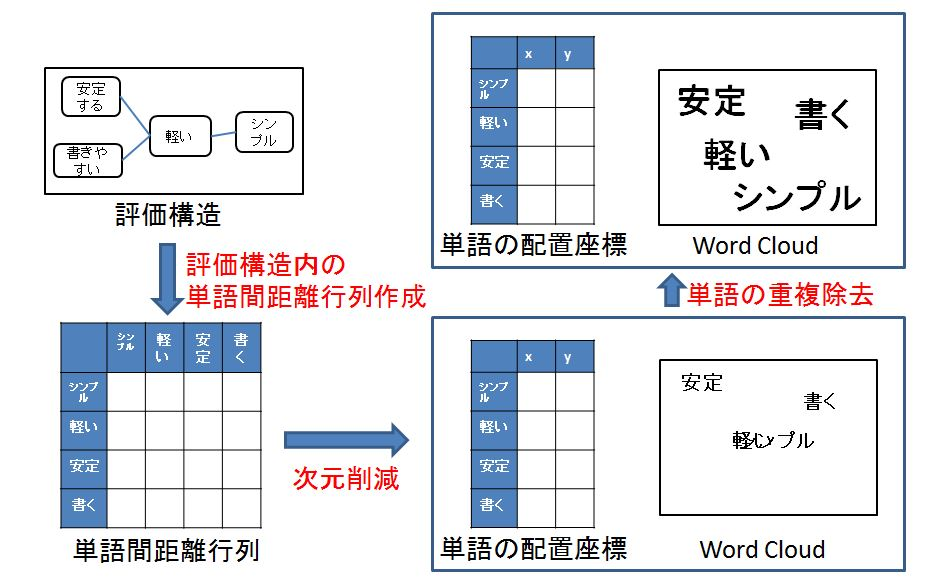
\includegraphics[width=\linewidth]{./png/met1.JPG}
				}
			\end{center}
			\caption{提案手法による可視化手順}
	  		\label{fig:met1}
		\end{figure}
		\begin{figure}
			\begin{center}
				\fbox{
				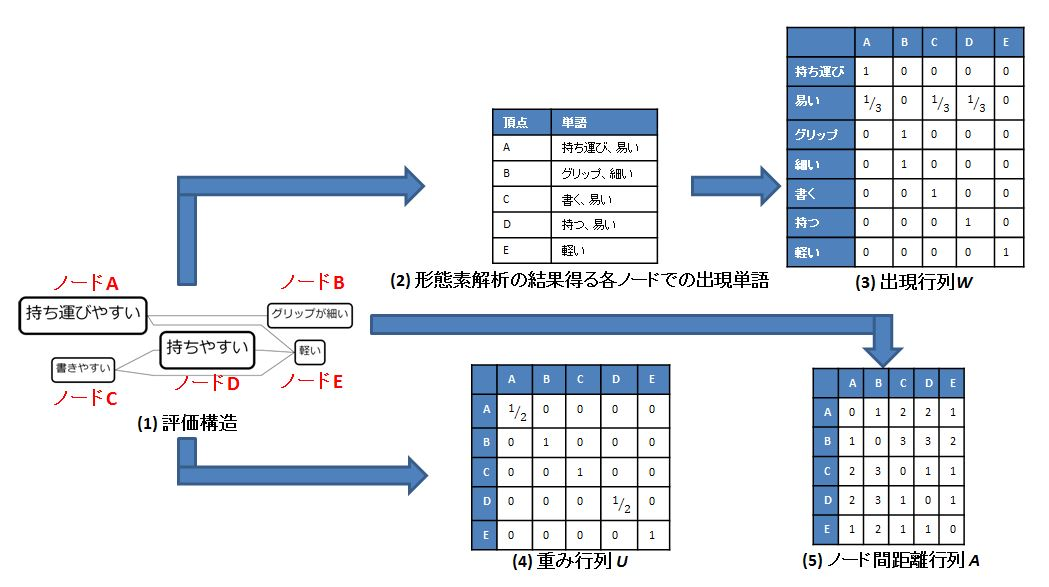
\includegraphics[width=\linewidth]{./png/met2.JPG}
				}
			\end{center}
			\caption{3行列の例}
	  		\label{fig:met2}
		\end{figure}
		\begin{figure}
			\begin{center}
				\fbox{
				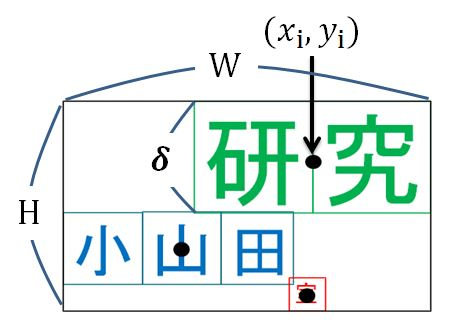
\includegraphics[width=\linewidth]{./png/met3.JPG}
				}
			\end{center}
			\caption{式(3.6)で使用される変数の例}
	  		\label{fig:met3}
		\end{figure}

%%提案システム
\chapter{提案システム}
	\section{システム要件}
		尾上が評価グリッド法の専門家のインタビュー結果を通して,評価構造分析システムの要件を分析した\cite{hak1}.
		先行研究で明らかにされた評価構造分析に求められている要件は以下のように要約される.
		\subsubsection{評価構造の全体を把握する}
			分析者はどのような単語や評価項目が評価構造内に現れているかに関心がある.
			頻出する単語,評価項目だけでなく一度しか出現しない単語,評価項目にも予想外の発見が存在する可能性はある.
			全体評価構造図を作成した後に,分析者は評価構造図を俯瞰し評価構造の全体像をつかむ.
			しかし,評価構造の規模が増大するに連れて評価構造の探索にかかる時間は増加し,
			評価項目や情報を見逃してしまう可能性もある.
			評価構造図をコンパクトに表示し,対話的な操作を可能にすることは,
			評価構造の全体把握を行う上では重要である.
		\subsubsection{評価項目間の関係性を把握する}
			評価項目の上位概念と下位概念を知ることは個人が持つ価値観の因果関係を知ることである.
			この因果関係は評価構造が持つ重要な情報の一つである.
			評価項目間の関係性を知るためには,分析者は注目した評価項目と隣接する評価項目を探索する.
			評価構造の規模が大きくなるにつれ,評価項目間の関係は複雑になり,評価項目間の関係性は把握しづらくなる.
			そのため評価構造図の読みやすさは重要な要素であり,その関係を確認するためのインタラクションが必要となる.
		\subsubsection{重要な項目を特定する}
			評価構造の中には複数人の実験参加者が回答した評価項目が存在する.
			この評価項目は,多くの人が共有している評価基準であり,
			分析者にとってこの評価項目を特定することは重要である.
			重要な評価項目を見つけるためには,重要な評価項目を自動的に絞り込むことや強調表示することが必要となる.
		\subsubsection{評価項目をグループ分けする}%%%尾上さんにグループ分けが必要な理由を聞きそれを記述
			評価構造内の評価項目をグループ分けすることは分析において必要である.
			従来は,分析者が主観的に評価項目を分類し,グループを作成していたが,
			分析者の主観が入る場合があり,分析者によってグループ分けの結果が異なる場合がある.
			そのため,客観的な基準をもとにグループ分けを行う機能は必要である.
	\section{システム設計と実装}
		前節で述べたシステム要件をもとに,評価構造分析システムの開発を行った.
		本節では提案システムの設計と実装の詳細について述べる.
		\subsection{概要}
			図~\ref{fig:sys1}は提案システムのスクリーンショットである.
			提案システムは3つの要素から構成されており,それぞれ評価構造ウィンドウ,Word Cloudウィンドウ,評価項目リストウィンドウである.
			図~\ref{fig:sys1}の右側に配置されているウィンドウが評価構造ウィンドウである.
			評価構造ウィンドウは評価構造図をネットワークで表示し,このウィンドウの目的は,評価構造内の評価項目間の関係性を直接見ることである.
			評価構造ウィンドウはWord Cloudウィンドウ,評価項目リストウィンドウと連動していて,
			あるウィンドウでの操作が即座に他のウィンドウに反映される.
			図~\ref{fig:sys1}の左側に配置されているウィンドウがWord Cloudウィンドウである.
			Word Cloudウィンドウでは提案手法を用いた評価構造内の評価項目で使用されている単語を表示する.
			Word Cloudウィンドウでの目的は,重要な単語の発見や,単語間の概括的な関係性の発見,評価構造の概要把握が挙げられる.
			図~\ref{fig:sys1}の左下側に配置されているウィンドウが評価項目リストウィンドウである.
			評価項目リストウィンドウではWord Cloudウィンドウで選択した単語が使用されている評価項目を表示する.
			評価項目リストウィンドウの目的は,ユーザーが単語に注目した場合の詳細な情報を示すことである.
			提案システムの評価構造ウィンドウと評価項目リストウィンドウはE-Gridから得た評価構造データを用いて表示し,
			Word CloudウィンドウはE-Gridから得た評価構造データと提案手法を用いて作成したデータを用いて表示した.
			
			提案システムはHTMLやJavaScriptといったWeb標準技術を用いて開発されたWebアプリケーションである.
			また,レイアウトの一部はbootstrapを用いて実装しており,タブレット端末のような画面の小さい装置や
			PCディスプレイ,タイルドディスプレイのような大画面好解像度での柔軟なレイアウトを可能にしている.
			
			提案システムの機能は以下のようにシステム要件を満たしている.
			\subsubsection{評価構造の全体を把握する}
				ユーザーはWord Cloudウィンドウを見ることで評価構造の概要を把握することができる.
				頻出単語は大きく表示され,そうでない単語も助詞や助動詞などの意味なし語を表示しないため,
				ネットワーク図で全体を表示した場合よりも大きいフォントサイズで表示される.
			\subsubsection{評価項目間の関係性を把握する}
				ユーザーはWord Cloudウィンドウ内の単語の位置関係から評価項目内の単語間の関係を把握することができる.
				また,その中から注目したい単語を選択することで,注目した単語と共起する単語,
				評価構造内で隣接関係にある評価項目の単語を知ることができる(図~\ref{fig:sys2}).
				また,Word Cloudウィンドウ内で単語を選択することで,評価項目リストウィンドウでは選択単語が使用されている
				評価項目がリスト表示され,評価構造ウィンドウでは選択単語が使用されている
				評価項目が強調される.
			\subsubsection{重要な項目を特定する}
				Word Cloudウィンドウ内の単語のフォントサイズは評価構造内での単語の出現頻度と比例して大きくなるので,
				ユーザーはWord Cloudウィンドウ内のフォントサイズを確認することで重要な項目を発見することができる.
			\subsubsection{評価項目をグループ分けする}%%%尾上さんにグループ分けが必要な理由を聞きそれを記述
				ネットワーク図での単語の距離関係をもとにWord Cloudでの単語座標を決定しているので,
				隣接する評価項目の単語が近くに配置されることが多い.これにより,
				ユーザーはWord Cloudウィンドウ内の単語の配置を確認することで,
				グループ分けを行うことが可能である.
			
		\subsection{ユーザインタラクション}
			提案システムでは主に2種類のユーザインタラクションを実装している.
			1つ目はWord Cloud内単語の評価構造内での関係性を表示するための単語選択,
			2つ目はWord Cloud内単語の評価構造内での関係性の絞り込みを行うためのリスト内チェックボックス選択である.
			
			1つ目のインタラクションは,Word Cloudウィンドウで発見した注目したい単語の詳細情報を知るための機能である.
			注目したい単語を選択,もしくはマウスオーバーすることで3つのウィンドウが連動し表示画面が変化する.
			単語をマウスオーバーすると,評価構造ウィンドウでマウスオーバーされた単語が使用されている評価項目が赤色で強調される.
			次に,単語を選択すると,Word Cloudウィンドウでは選択した単語の評価構造内での関係性を表示する.
			選択単語と評価項目内で共起している単語が紫色に変化し,
			選択単語が使用されている評価項目と隣接する評価項目内の単語が青色,もしくは赤色に変化する.
			選択単語が使用されている評価項目の上位概念の評価項目の単語は青色,下位概念の評価項目の単語は赤色で表示される.
			それ以外の単語は不透明度を下げることで,注目単語の情報のみを表示するようにした.
			同時に,選択単語と選択単語が使用されている評価項目と隣接する評価項目内の単語をエッジで結ぶ.
			エッジの色について選択単語が使用されている評価項目の上位概念の評価項目の単語と結ぶ線は青色,
			下位概念の評価項目の単語と結ぶ線は赤色で表示される.
			評価項目リストウィンドウでは,選択単語が使用されている評価項目を表示することで評価項目の情報を示す.
			評価構造ウィンドウでは,選択単語が使用されている評価項目とその上位及び下位概念の評価項目が強調される.
			選択単語が使用されている評価項目は紫色,選択単語が使用されている評価項目の上位及び下位概念はそれぞれ青色,赤色で強調される.
			これによって注目単語と関係をもつ評価項目と単語の詳細を把握することができる.
			
			また,2つ目のインタラクションは1つ目のインタラクションを使用した後に使えるようになる.
			2つ目のインタラクションは,選択単語が複数の評価項目で使用されている場合に,その中の特定の評価項目が評価構造内のどこにあるのか,
			その上位及び下位概念の評価項目は何であるかを知りたい際に使用される.
			評価項目リストウィンドウ内で,詳細を知りたい評価項目の列のチェックボックスを選択することで,
			評価構造ウィンドウでは,選択評価項目,その上位及び下位概念の評価項目のみが強調される.
			同時にWord Cloudウィンドウでも,選択評価項目,その上位及び下位概念の評価項目の単語のみが強調される.
			
			これら2種類のインタラクションによりユーザーは注目した単語や評価項目の詳細情報を対話的な操作から得ることができる.
			
		\begin{figure}
			\begin{center}
				\fbox{
				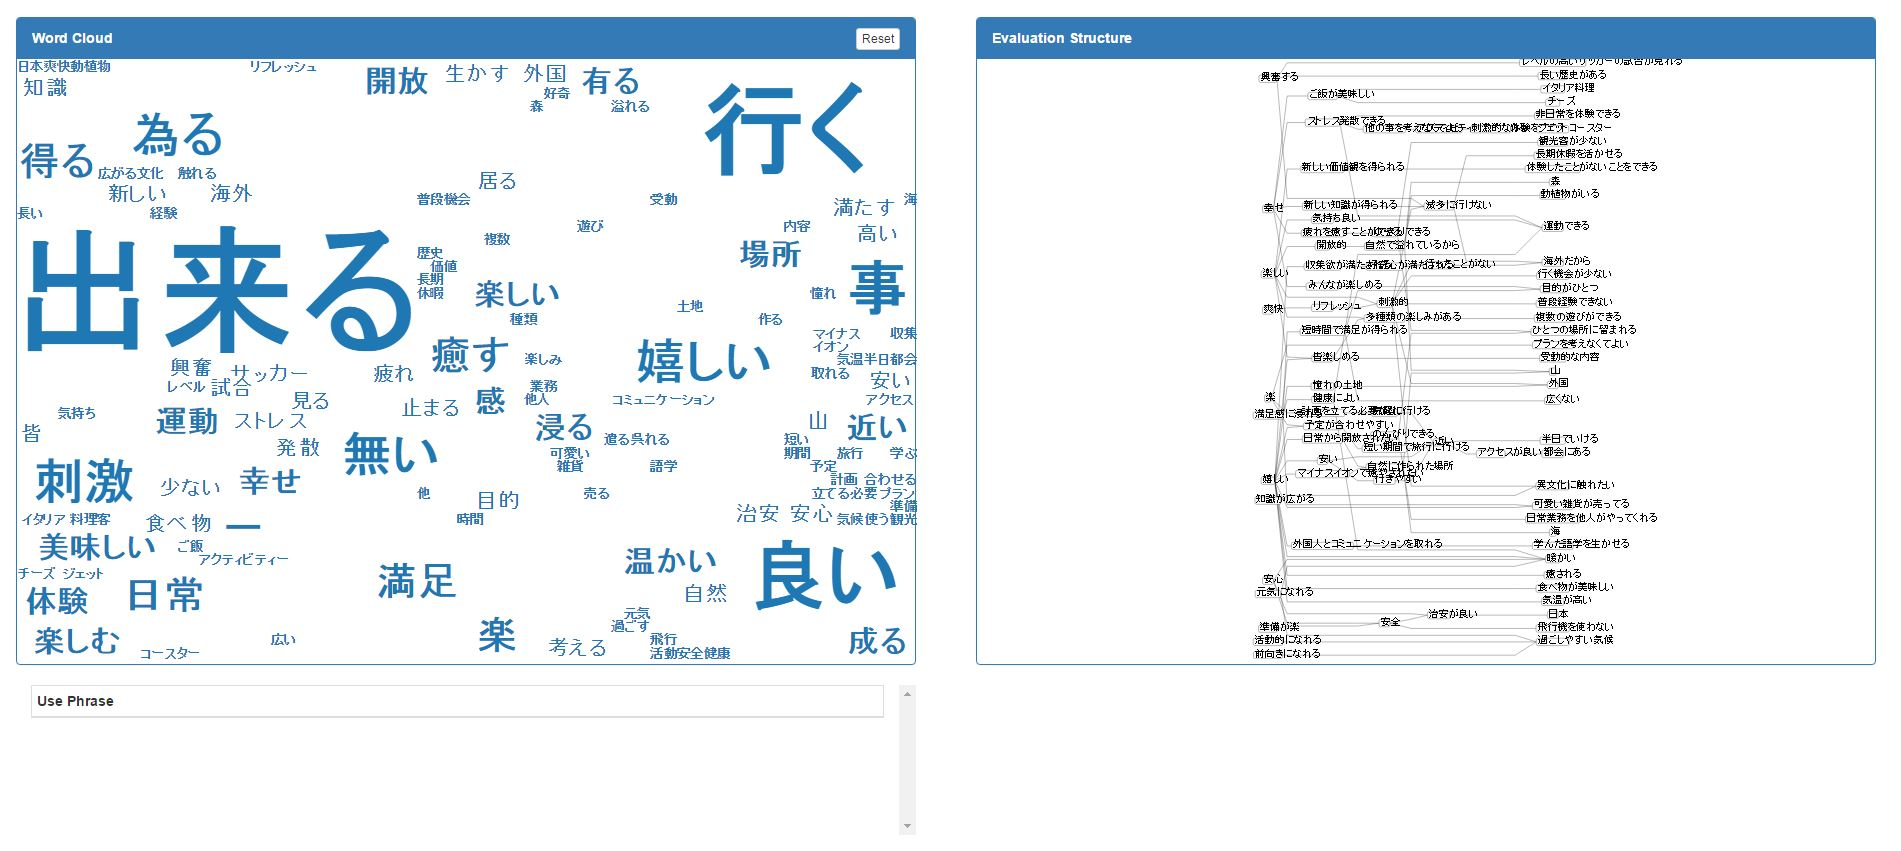
\includegraphics[width=\linewidth]{./png/sys1.JPG}
				}
			\end{center}
			\caption{提案システムの概要}
	  		\label{fig:sys1}
		\end{figure}
		\begin{figure}
			\begin{center}
				\fbox{
				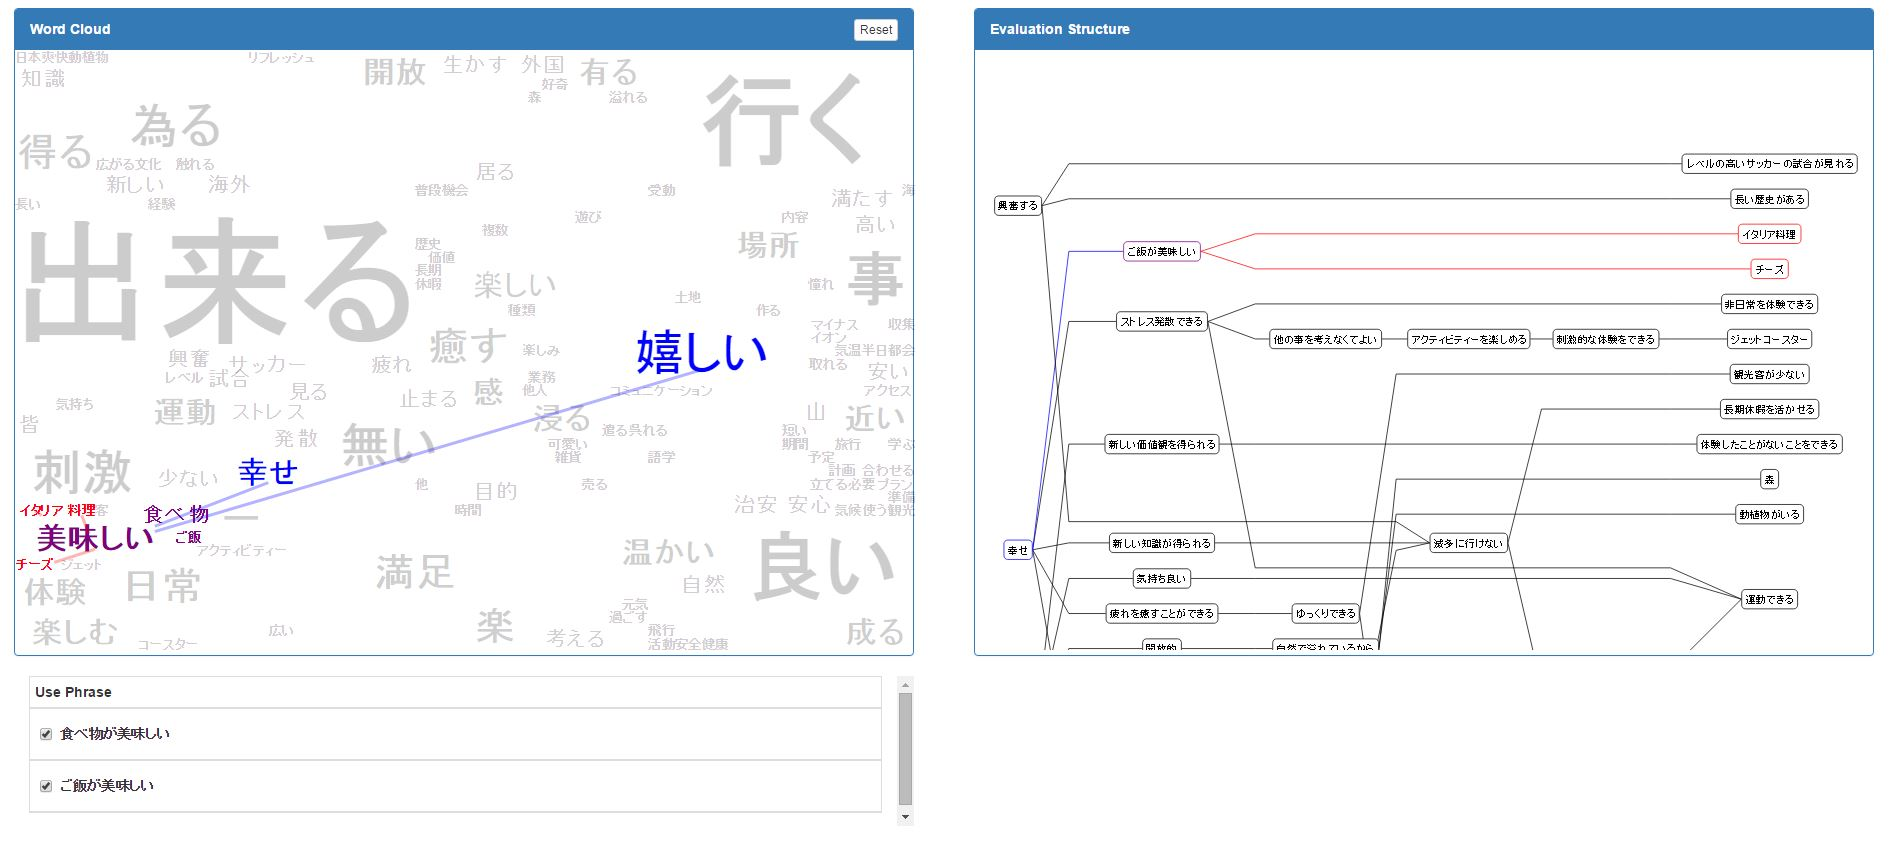
\includegraphics[width=\linewidth]{./png/sys2.JPG}
				}
			\end{center}
			\caption{提案システムの概要2}
	  		\label{fig:sys2}
		\end{figure}

%%評価実験
\chapter{評価実験}
	本章では,提案手法,提案システムの有効性を証明するために行った2組の比較実験とケーススタディ,ユーザーフィードバックの評価実験について述べる.
	Word Cloud可視化とWord Cloud内単語の配置座標を計算したことの評価を行うために比較実験とユーザーフィードバックを行った.
	また,提案システムが評価構造分析に有効であることを証明するためにケーススタディを行った.
	\section{比較実験}
		\subsection{比較対象}
			実験では,2組の比較実験を行った.
			1組目は提案手法によるWord Cloud表示(Nword Cloud)と従来のネットワーク表示(ネットワーク図)の比較である.
			この比較実験により,Word Cloudによる可視化の有効性を証明する.
			2組目はNword Cloudと,配置座標をランダムに決定したWord Cloud表示(Rword Cloud)との比較結果を行った.
			こちらの比較実験ではWord Cloud内の単語の配置座標を考慮することの有効性を証明する.
			
			比較実験で使用するネットワーク図のインタラクションは前章で説明した内容の中で,
			ネットワーク図とWord Cloud間の連携部分以外は実装されている.
			Nword Cloud,Rword Cloudのインタラクションは前章のWord Cloudウィンドウで説明した内容の中で,
			ネットワーク図とWord Cloud間の連携部分以外は実装されている.
			また,Nword CloudとRword Cloudには評価項目リスト画面が実装されている.
			図~\ref{fig:que1}はネットワーク図,図~\ref{fig:que2}はNword Cloud,
			図~\ref{fig:que3}はRword Cloudの例である.
			
		\subsection{実験データ}
			実験には3種類の評価構造データを使用する.
			評価構造のデータとして,E-Gridを使用したインタビュー結果から得られたデータを使用した.
			インタビューは日本語で,回答者と質問者の1対1で行われた.
			評価項目数はそれぞれ15個,45個,136個の3種類用意した.
			評価項目数が15個のデータは,乗りたい自動車についての評価構造である.
			このデータは1人の回答者の評価構造であり,形態素解析によって得た37個の形態素をNword CloudとRword Cloudで表示した.
			評価項目数が45個のデータは,行きたい旅行先についての評価構造である.
			このデータは3人の回答者の評価構造を統合した全体評価構造であり,形態素解析によって得た70個の形態素をNword CloudとRword Cloudで表示した.
			評価項目数が136個のデータは,欲しいシャープペンシルについての評価構造である.
			このデータは16人の回答者の評価構造を統合した全体評価構造であり,形態素解析によって得た172個の形態素をNword CloudとRword Cloudで表示した.
		
		\subsection{実験内容}
			3種類の評価構造データの可視化に対してそれぞれ3種類のタスクを用意した.
			実験内容はシステム要件で述べられた,評価構造分析に求められる3つの機能を考慮して作成した.
			\begin{enumerate}
				\item 評価構造の全体を把握する
				\item 評価項目,単語の関係性を把握する
				\item 重要な項目を特定する
			\end{enumerate}

			タスク1では,評価構造内に存在する評価項目を4つの選択肢から選択させる.
			このタスクでは,評価構造分析に求められる機能の1つ目である評価構造の全体把握への有効性を評価するために,
			評価構造内で頻出する評価項目だけでなく,1度しか回答されていない評価項目など様々な評価項目を正解の選択肢に選定した.
			タスク2では,特定の単語が使用されている評価項目と隣接する評価項目内の単語を選択させる.
			このタスクでは,評価構造分析に求められる機能の2つ目である評価項目や単語の関係性の把握への有効性を評価するため行う.
			タスク3では,評価構造内で基も多く使用されている単語を4つの選択肢から選択させる.
			このタスクでは,複数人が共有する評価基準を探索させることから,評価構造分析に求められる機能の3つ目である重要な項目の特定への有効性を評価した.
			
			実験用のプログラムはWebベースで開発を行い,結果の記録や問題の生成を自動化した.
			図~\ref{fig:que1}はタスク1,図~\ref{fig:que2}はタスク2,
			図~\ref{fig:que3}はタスク3のページのスクリーンショットである.
			評価指標としてタスクの所要時間,タスクの正答率を使用した.
		
		\subsection{実験手順}
			実験参加者は10人である.
			はじめに評価構造のネットワーク図とNword Cloud,Rword Cloudの特徴を説明し,
			サンプルシステムを通してシステムの使用法を学ばせた.
			説明の後にタスクの内容説明と例を示し,3種類の評価構造を3種類の可視化手法を用いて表示したタスク計9個を行わせた.
			実験参加者毎に選択肢を生成し,順番に実行するように指示をした.
			実験には,ネットワーク図が画面内に収まる十分な大きさのディスプレイと使い慣れたポインティングデバイスを使用するように指示をした.
		
	\section{ケーススタディ}
		本節では,提案システムの使用例を通じた評価を行う.
		提案システムを用いたケーススタディを1名が行い,提案システムで評価構造の頻出語や頻出語から帰結する評価基準の探索を行った.
		実験に使用した機材はCPU がIntel Core i3,メモリが4.00GB,OSがwindows 8.1,ディスプレイは10.6インチ液晶ディスプレイ,解像度1920×1080のPC である.
		提案システムはGoogle Chromeから使用した.
		参加者にはシステムの使用方法について事前にサンプルデータを用いたシステムを見せて説明した.以下では実験に使用したデータについて述べる.
		
		このケーススタディでは,「行きたい旅行先」に関する調査で得られた全体評価構造を使用した.
		全体評価構造は7人の被験者による評価構造から構成される.
		評価構造はE-Gridを使用したインタビューによって作成された.
		インタビューは日本語で,被験者と質問者の1対1で行われた.
		刺激要素として,被験者が行きたい旅行先をそれぞれ4つ使用した.
		インタビューの結果89個の評価項目と103個の評価項目間の接続による全体評価構造が得られた.
		被験者らは,旅行計画を考えており,その際に多くの旅行参加者の希望をかなえた旅行計画を作成するために提案システムを使用した.
		Word Cloudでは評価構造のテキストデータの中から名詞,動詞,形容詞を抽出して可視化した.
		また,名詞のうち数字は除外した.
		ケーススタディ参加者には,実験後に提案システムの有効な点や改善が必要な点,追加すべき機能など自由記述アンケートを行った.
		
	\section{ユーザーフィードバック}
		比較実験後に10名の参加者にはシステムに関するアンケートを行った.
		アンケートでは3種類の可視化手法について5段階評価させた.
		アンケートの項目は以下の3つである.
		
		\begin{itemize}
			\item 新しい発見や仮説構築につながる示唆が得られそうか
			\item 多くの人が共有する評価項目を発見することに有効であるか
			\item 評価項目間の因果関係を発見することに有効であるか
		\end{itemize}
		また,アンケートと同時にNword Cloudについて自由記述のアンケートも実施した.
		
		\begin{figure}
			\begin{center}
				\fbox{
				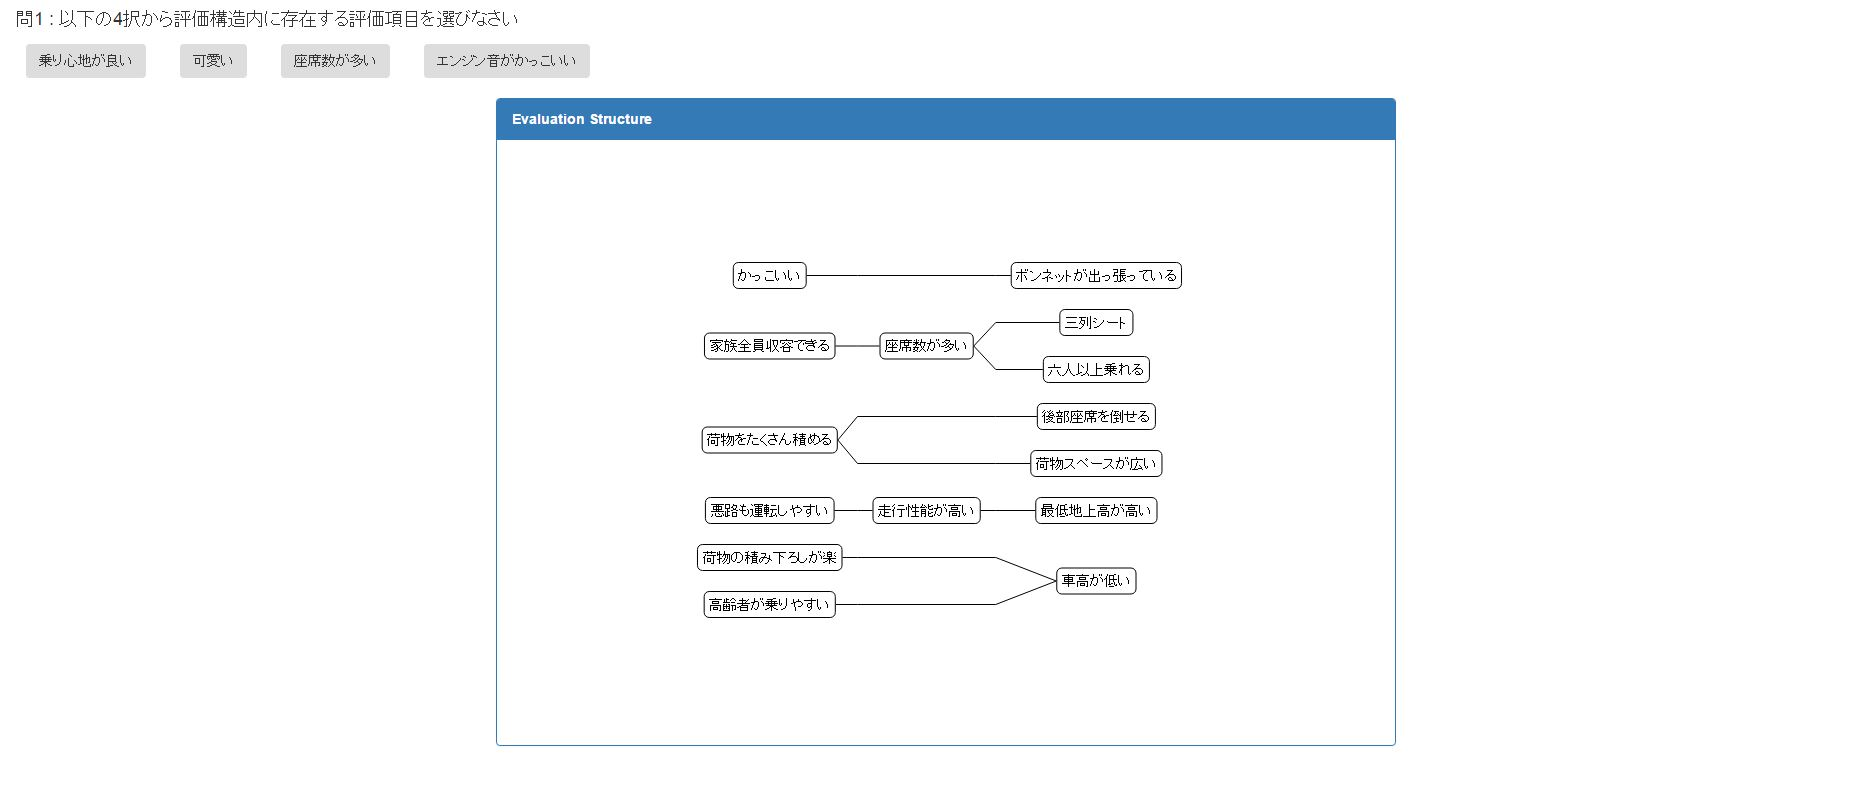
\includegraphics[width=\linewidth]{./png/que1.JPG}
				}
			\end{center}
			\caption{ネットワーク図によるタスク1の例}
	  		\label{fig:que1}
		\end{figure}
		\begin{figure}
			\begin{center}
				\fbox{
				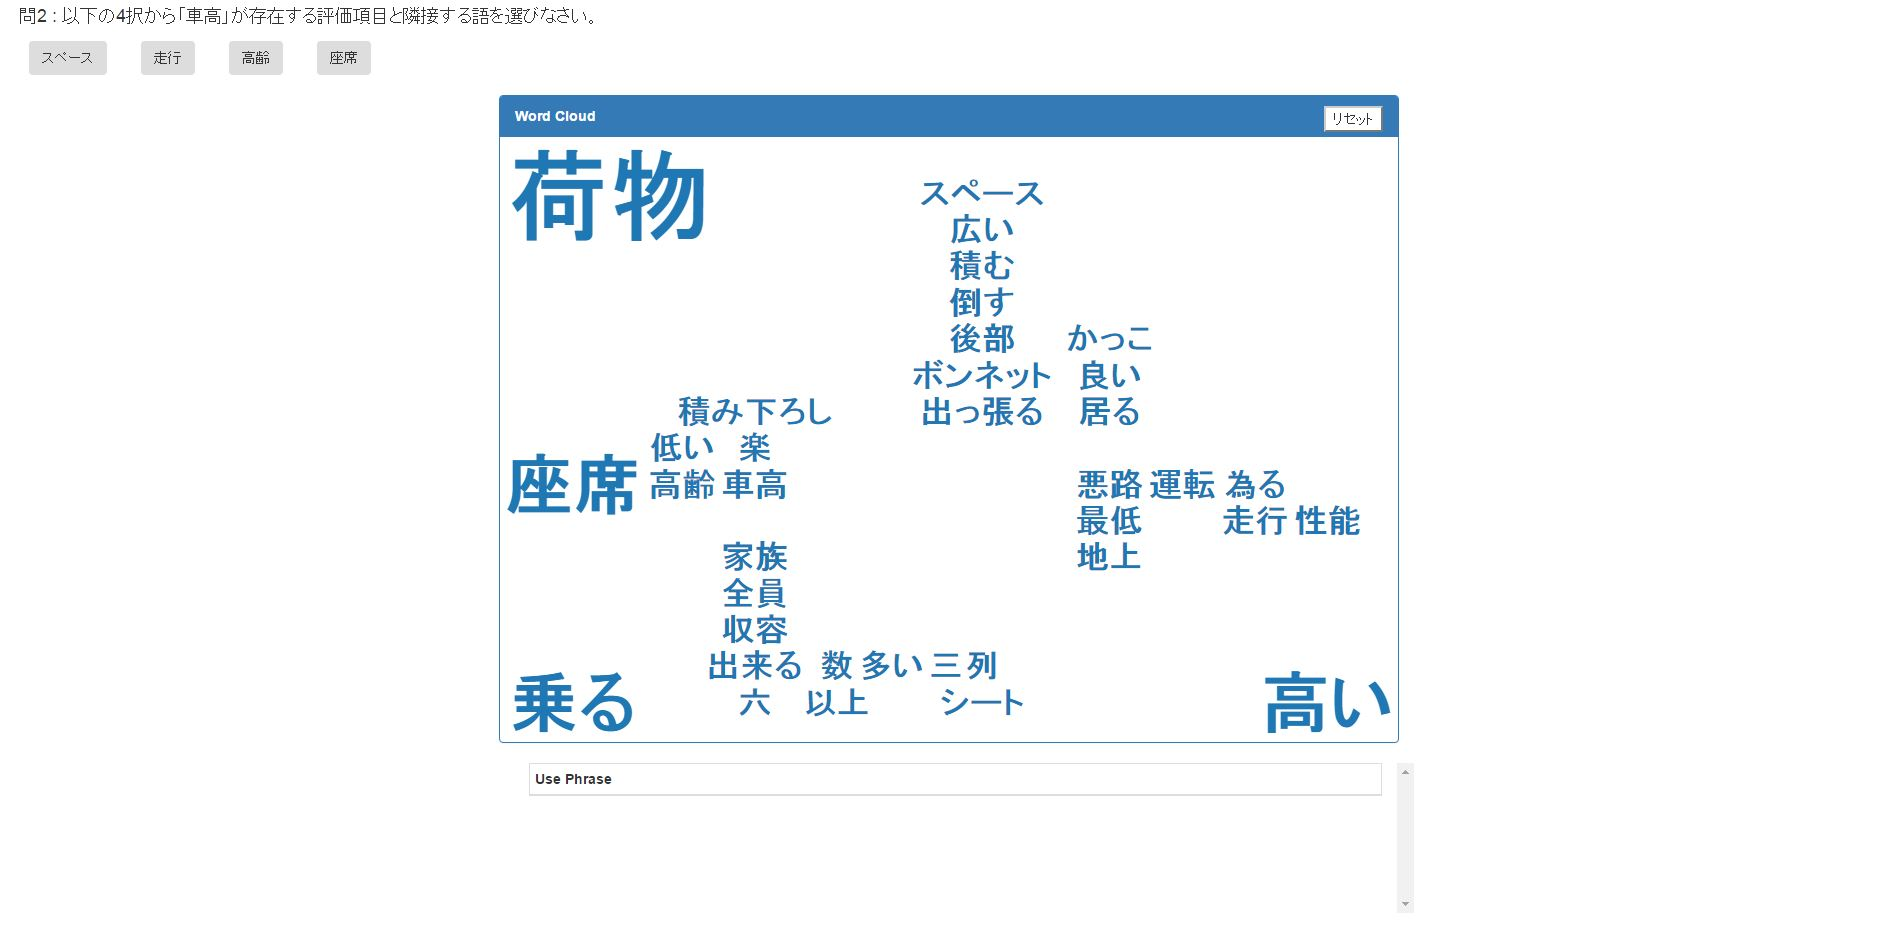
\includegraphics[width=\linewidth]{./png/que2.JPG}
				}
			\end{center}
			\caption{Nword Cloudによるタスク2の例}
	  		\label{fig:que2}
		\end{figure}
		\begin{figure}
			\begin{center}
				\fbox{
				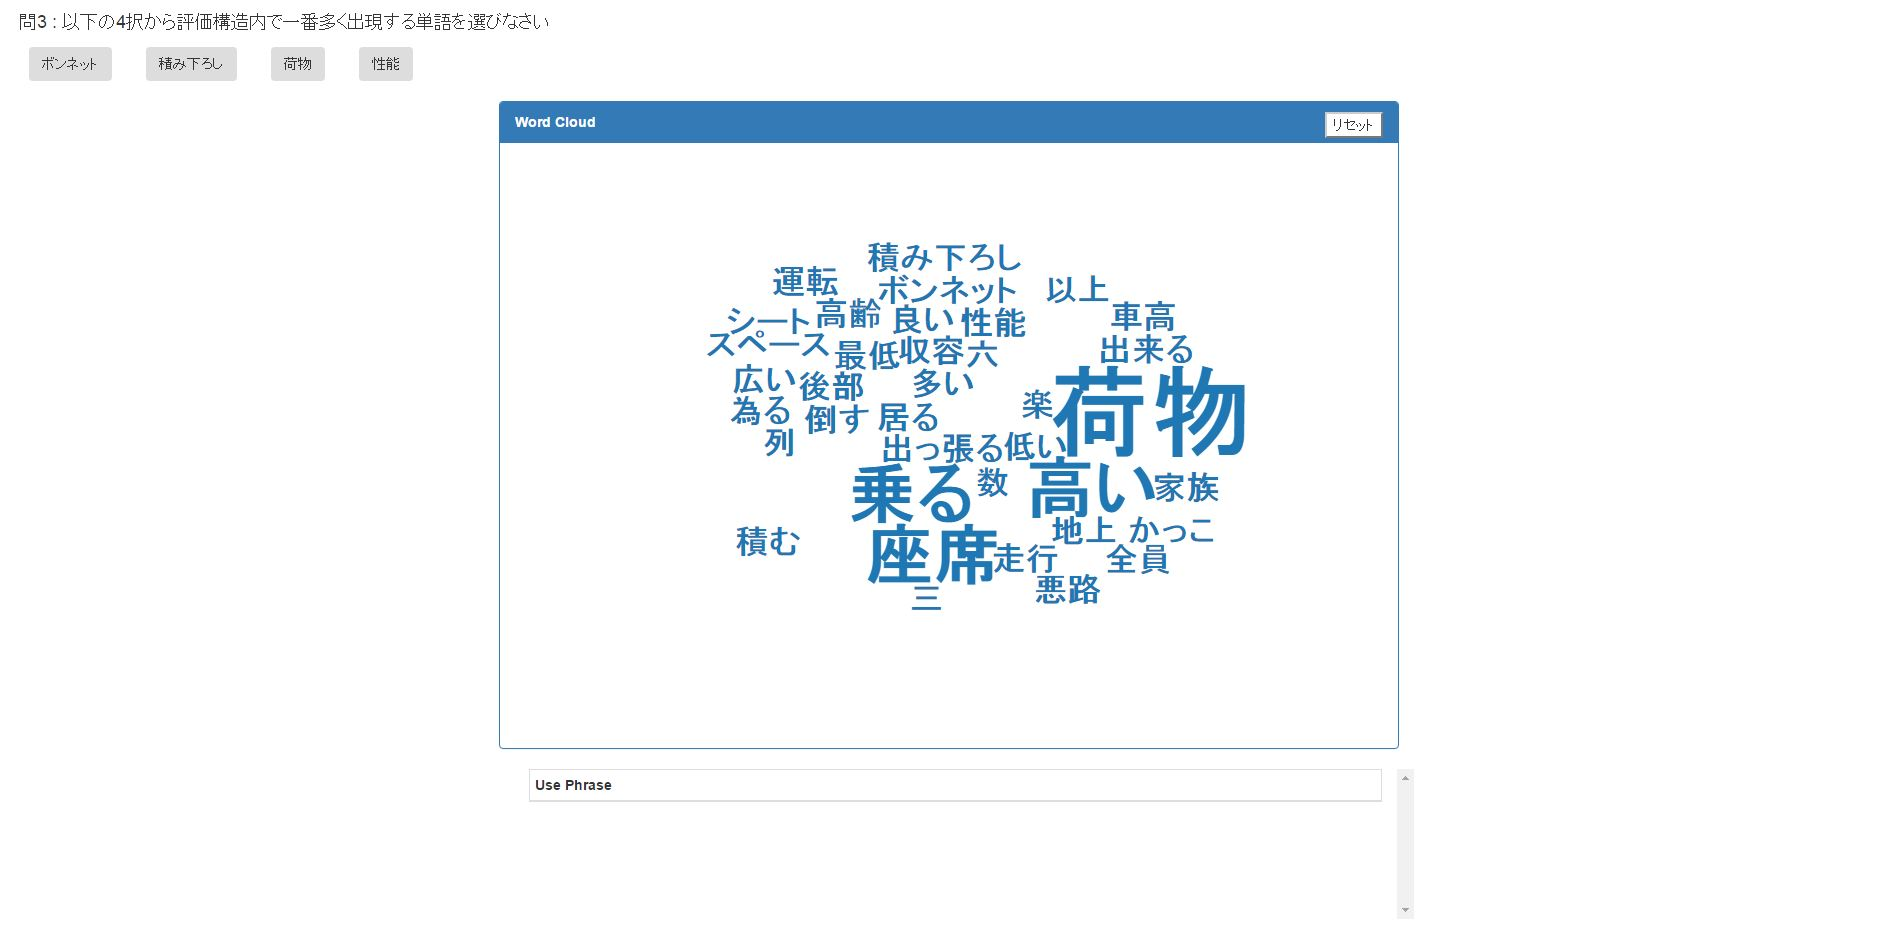
\includegraphics[width=\linewidth]{./png/que3.JPG}
				}
			\end{center}
			\caption{Rword Cloudによるタスク3の例}
	  		\label{fig:que3}
		\end{figure}

%%実験結果
\chapter{実験結果}
	\section{比較実験}
	%%%ノード数まとめた 平均時間正答率 棒グラフ
	ここでは,3種類の可視化手法によるタスクの平均所要時間,平均正答率の結果について述べる.
	タスク1の平均所要時間の結果を図~\ref{fig:res1}に表す.
	タスク1の平均所要時間について,ノード数が15個の場合では差が少ないが,ノード数が136個の場合ではネットワーク図がWord Cloud表示の約3倍以上の時間を要した.
	Nword Cloudと他の可視化手法間の平均所要時間に有意差があるか確認するためにt検定を用いたところ,
	ノード数が136個の場合にP値が0.012と棄却域を下回っており,有意差があると判定された.
	タスク2の平均所要時間の結果を図~\ref{fig:res2}に表す.
	タスク2の平均所要時間は,Nword Cloudが他の可視化手法と比較すると短く,
	ノード数が136個の場合では他の可視化手法の半分以下の時間であった.
	Nword Cloudと他の可視化手法間で平均所要時間に有意差があるか確認するためにt検定を用いたところ,
	Nword CloudとRword Cloud間ではノード数が136個の場合にP値が0.004と棄却域を下回っており,有意差があると判定された.
	タスク3の平均所要時間の結果を図~\ref{fig:res3}に表す.
	タスク3の平均所要時間は,ノード数に関係なくネットワーク図が最も長かった.
	Nword Cloudと他の可視化手法間で平均所要時間に有意差があるか確認するためにt検定を用いたところ,
	ノード数が15個の場合のNword Cloudとネットワーク図間以外では有意差が確認できなかった.
	
	タスクの平均正答率については,図~\ref{fig:res4},図~\ref{fig:res5},図~\ref{fig:res6}のようにノード数,可視化手法によってあまり差は見られなかった.
	全タスクでの正答率はRword Cloudが一番高かったが,
	他の可視化手法との正答率の有意差についてt検定を用いて確認したところ,全てのノード数で有意差は確認できなかった.
		
	\section{ケーススタディ}
	評価構造の分析は,評価構造作成の際の被験者3人によって行われた.
	分析の対象である評価構造データを使用した提案システムのスクリーンショットを図~\ref{fig:sys1}に表す.
	はじめに,評価構造に含まれる単語を概観するためにWord Cloudウィンドウを確認した.
	フォントサイズの大きい単語から注目したい単語を探し,そこから分析者は「癒す」,「疲れ」という慰安目的の旅行や,
	「美味しい」,「料理」,「食べ物」など食べあるき旅行,「運動」,「ストレス」,「発散」など体を動かす旅行などを求めている,
	また,これらの単語の中で「癒す」のフォントサイズが一番大きいことから慰安目的の旅行を求めている人が多いのではないかという仮説を分析者らは立てた.
	
	次に,仮説を確認するため上記の単語の詳細な情報を探索した.
	分析者は「癒す」をクリックし,評価項目リストウィンドウから「癒す」が使用されている評価項目を確認した(図~\ref{fig:cas1}).
	「癒す」は「マイナスイオンで癒やされたい」,「癒される」,「疲れを癒やすことができる」という評価項目で使用されていた.
	その中で,「マイナスイオンで癒やされたい」の詳細について分析者らは興味を持った.
	
	次に,上位及び下位の評価項目を探索した.
	分析者は評価項目リストウィンドウの「マイナスイオンで癒やされたい」以外のチェックボックスを外し,
	ネットワーク図内で評価項目の絞り込みを行った(図~\ref{fig:cas2}).
	「マイナスイオンで癒やされたい」の評価項目は紫色,上位に接続されたエッジと評価項目は青色,
	下位に接続されたエッジと評価項目は赤色で強調表示されている.
	ネットワークウィンドウからは「マイナスイオンで癒やされたい」ことの好ましい理由として「嬉しい」という上位項目が得られた.
	同様に,「マイナスイオンで癒やされたい」ための条件として「自然で尽きられた場所」,「海」「山」という下位項目が得られた.
	
	このケーススタディによって,提案システムでは対話的な操作によって評価構造の効果的な分析が可能であることが示された.
	提案システムでは,従来のネットワーク図のみでは発見が困難であった多くの人が共有する頻出語,頻出語と因果関係を持つ単語の発見を促進し,
	評価構造の概観の効率化を行った.
	
	\section{ユーザーフィードバック}
		\subsection{5段階評価アンケート結果}
		この項では5段階評価アンケートの結果について述べる.
		「新しい発見や仮説構築に繋がる示唆は得られそうか」についての評価は,図~\ref{fig:res7}のように
		ネットワーク図,Nword Cloud,Rword Cloudの順になった.
		3可視化手法間の評価の有意差を確認するためt検定を行ったが,有意差は確認できなかった.
		次に,「多くの人が共有する評価項目を発見することに有効であるか」についての評価は,
		図~\ref{fig:res8}のようにNword Cloud,Rword Cloud,ネットワーク図の順になった.
		3可視化手法間の有意差を検定するためにt検定を行ったところ,Nword Cloudとネットワーク図間ではP値が0.004となり棄却域を下回ったので,
		Nword Cloudでは多くの人が共有する評価項目の発見に有効であることが示された.
		最後に,「評価項目間の因果関係を発見することに有効であるか」についての評価は,
		図~\ref{fig:res9}のようにネットワーク図,Nword Cloud,Rword Cloudの順になった.
		3可視化手法間の有意差を検定するためにt検定を行ったところ,Nword CloudとRword Cloud間ではP値が0.040となり,
		棄却域を下回ったので,評価構造内の位置関係を考慮してWord Cloud内の単語の座標を決定することは評価項目間の因果関係を発見することに有効であることが示された.
	
		\subsection{自由記述アンケート結果}
		自由記述アンケート結果を以下に示す.
		\begin{itemize}
			\item ネットワーク図では拡大と移動を行わなければ文章を読み取ることができないが,Word Cloud表示ではそのような操作を必要とせず文章を概観することができる.
			\item 提案手法によるWord Cloud表示では,単語をクリックし関連する単語が強調表示される際に,ランダム配置と比較して,クリックした単語の近くに配置されていることが多いので単語間の関係性が読み取りやすいという点で優れている.
			\item 提案手法によるWord Cloud表示では,ランダム配置と比較して空白部分が多く,指定された単語を図中から探すことがやや難しかった.
			\item Word Cloud表示では,同じ大きさの単語が横に並べて配置された時に単語の切れ目を認識することが難しかった.
			\item 提案手法によるWord Cloud表示のほうが単語同士の距離が広くとられていて目的のノードを見つけやすかった.
			\item Word Cloud表示では,色と線が表示されるのがいい.ネットワーク図との連携があれば更に上位(下位)の項目をたどることが可能になると考えられる.
			\item ある特定の単語にマウスオーバーすることで,関連する単語が浮かび上がる動作は,明確な検索ワードを持ち合わせていないけれども探索を行いたい時にあると便利だと感じました.
			\item エッジがなくても,言葉の間のある程度の関係性が予想でき,そのあとエッジで確認することができるため,より自由な発想につながる可能性を感じました.
			\item 空白部分があるので全体的にフォントサイズを少し大きく出来るのではないかと感じました.
			\item テキスト入力した項目がクリックされる機能もほしい.
		\end{itemize}
		\begin{figure}
			\begin{center}
				\fbox{
				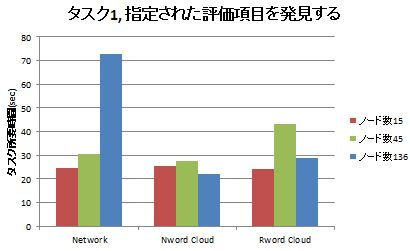
\includegraphics[width=\linewidth]{./png/res1.JPG}
				}
			\end{center}
			\caption{タスク1の所要時間}
	  		\label{fig:res1}
		\end{figure}
		\begin{figure}
			\begin{center}
				\fbox{
				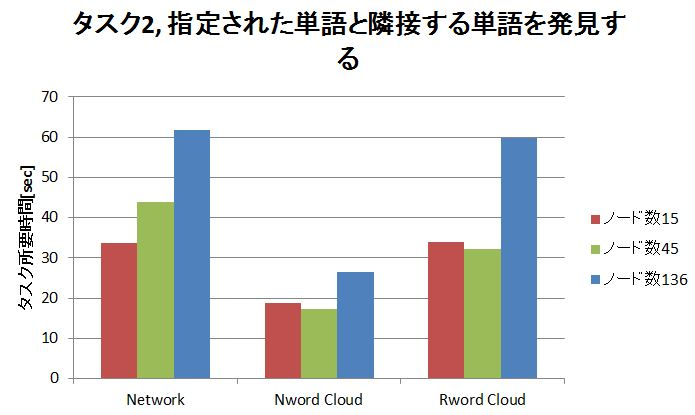
\includegraphics[width=\linewidth]{./png/res2.JPG}
				}
			\end{center}
			\caption{タスク2の所要時間}
	  		\label{fig:res2}
		\end{figure}
		\begin{figure}
			\begin{center}
				\fbox{
				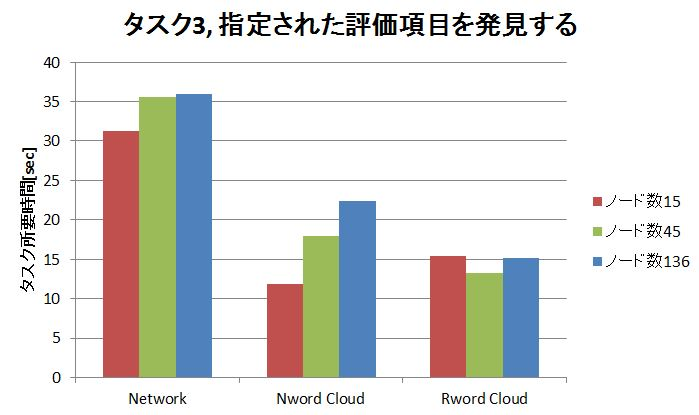
\includegraphics[width=\linewidth]{./png/res3.JPG}
				}
			\end{center}
			\caption{タスク3の所要時間}
	  		\label{fig:res3}
		\end{figure}
		\begin{figure}
			\begin{center}
				\fbox{
				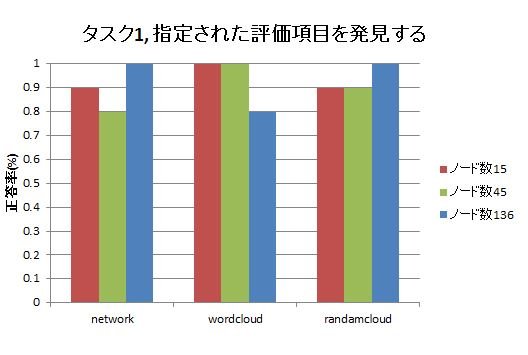
\includegraphics[width=\linewidth]{./png/res4.JPG}
				}
			\end{center}
			\caption{タスク1の平均正答率}
	  		\label{fig:res4}
		\end{figure}
		\begin{figure}
			\begin{center}
				\fbox{
				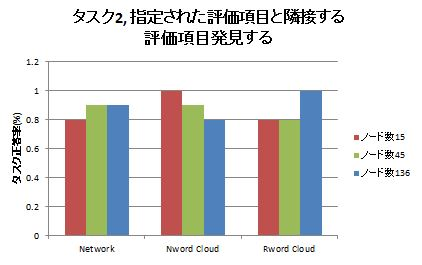
\includegraphics[width=\linewidth]{./png/res5.JPG}
				}
			\end{center}
			\caption{タスク2の平均正答率}
	  		\label{fig:res5}
		\end{figure}
		\begin{figure}
			\begin{center}
				\fbox{
				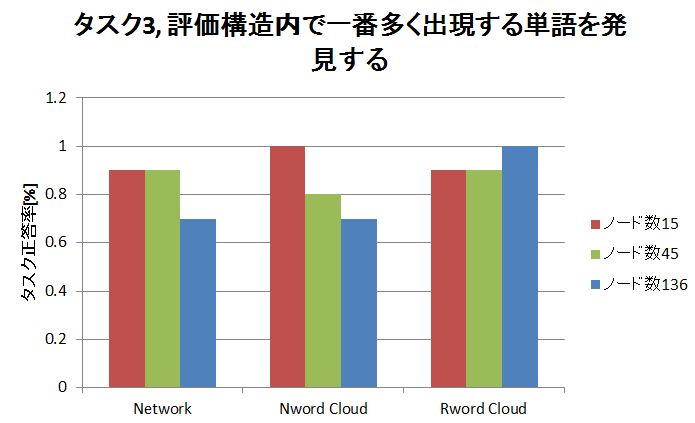
\includegraphics[width=\linewidth]{./png/res6.JPG}
				}
			\end{center}
			\caption{タスク3の平均正答率}
	  		\label{fig:res6}
		\end{figure}
		\begin{figure}
			\begin{center}
				\fbox{
				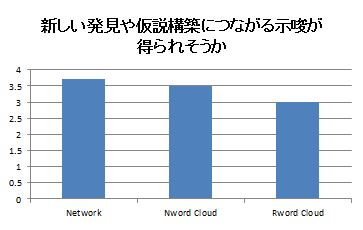
\includegraphics[width=\linewidth]{./png/res7.JPG}
				}
			\end{center}
			\caption{5段階評価アンケート結果1}
	  		\label{fig:res7}
		\end{figure}
		\begin{figure}
			\begin{center}
				\fbox{
				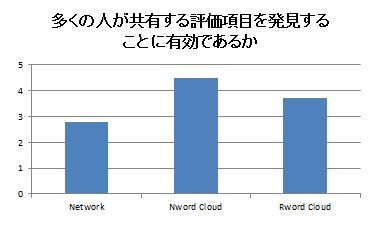
\includegraphics[width=\linewidth]{./png/res8.JPG}
				}
			\end{center}
			\caption{5段階評価アンケート結果2}
	  		\label{fig:res8}
		\end{figure}
		\begin{figure}
			\begin{center}
				\fbox{
				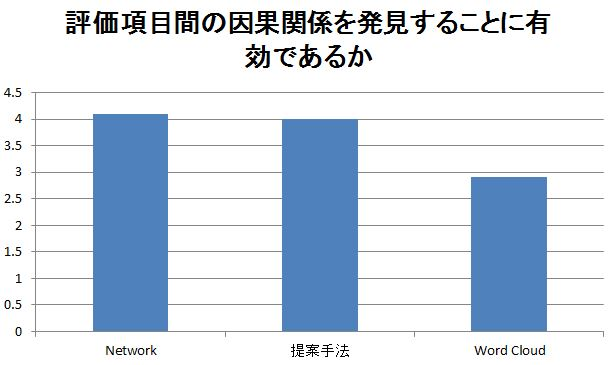
\includegraphics[width=\linewidth]{./png/res9.JPG}
				}
			\end{center}
			\caption{5段階評価アンケート結果3}
	  		\label{fig:res9}
		\end{figure}
		\begin{figure}
			\begin{center}
				\fbox{
				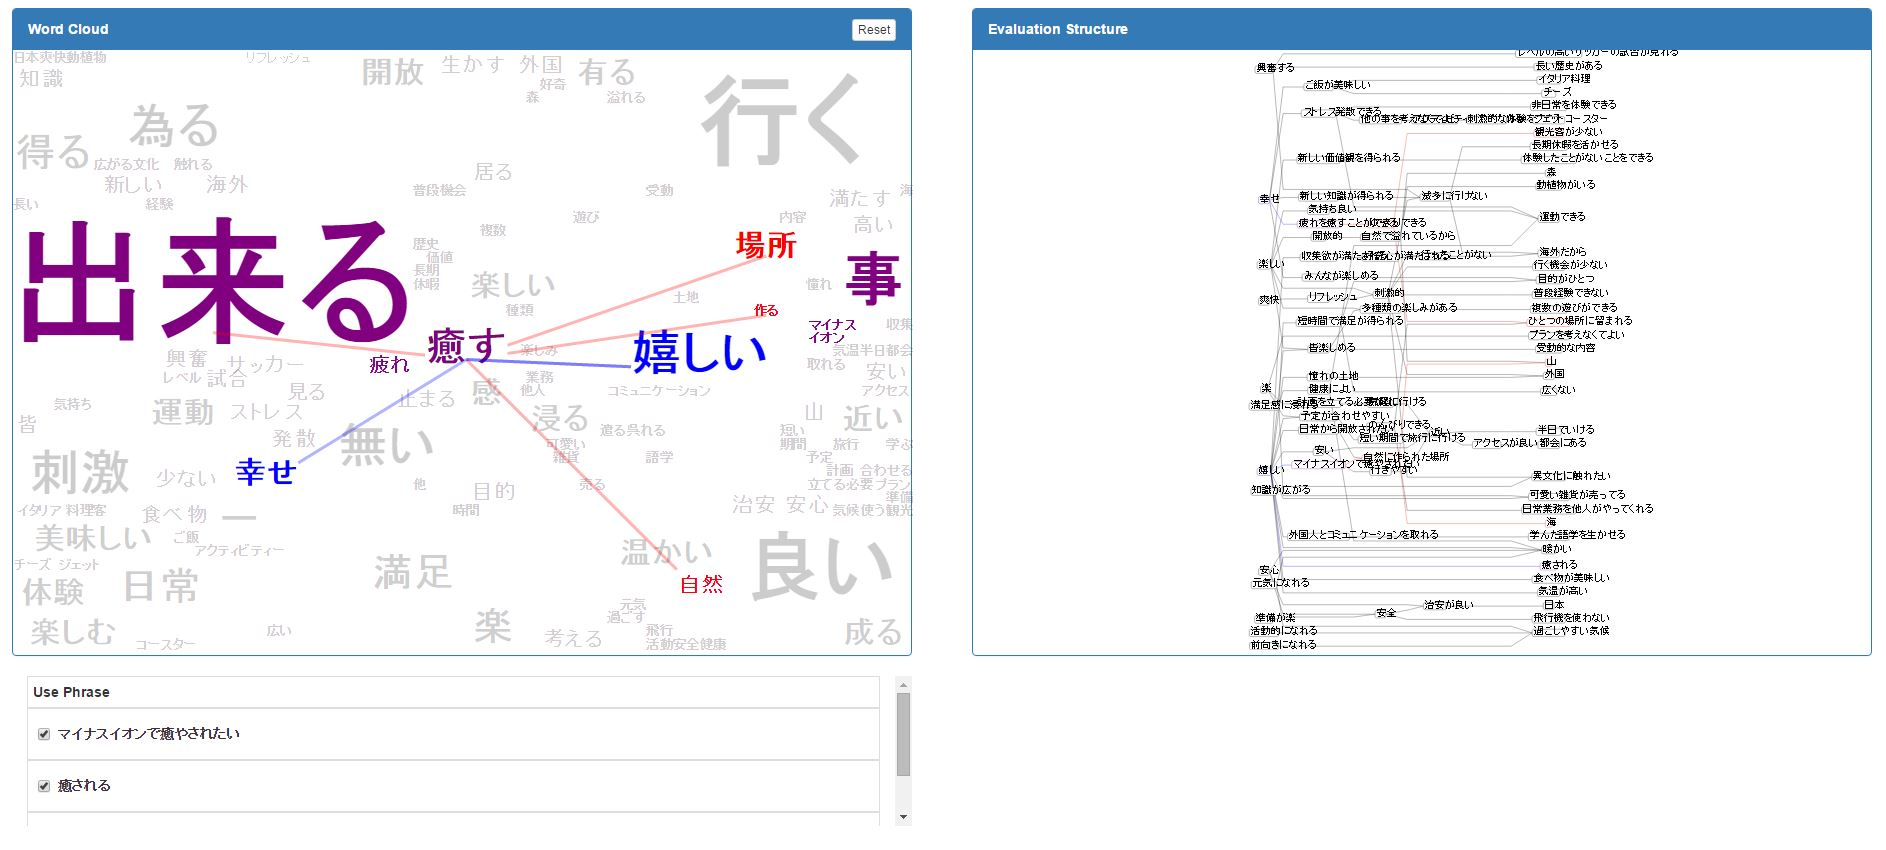
\includegraphics[width=\linewidth]{./png/cas1.JPG}
				}
			\end{center}
			\caption{注目単語の詳細情報の探索}
	  		\label{fig:cas1}
		\end{figure}
		\begin{figure}
			\begin{center}
				\fbox{
				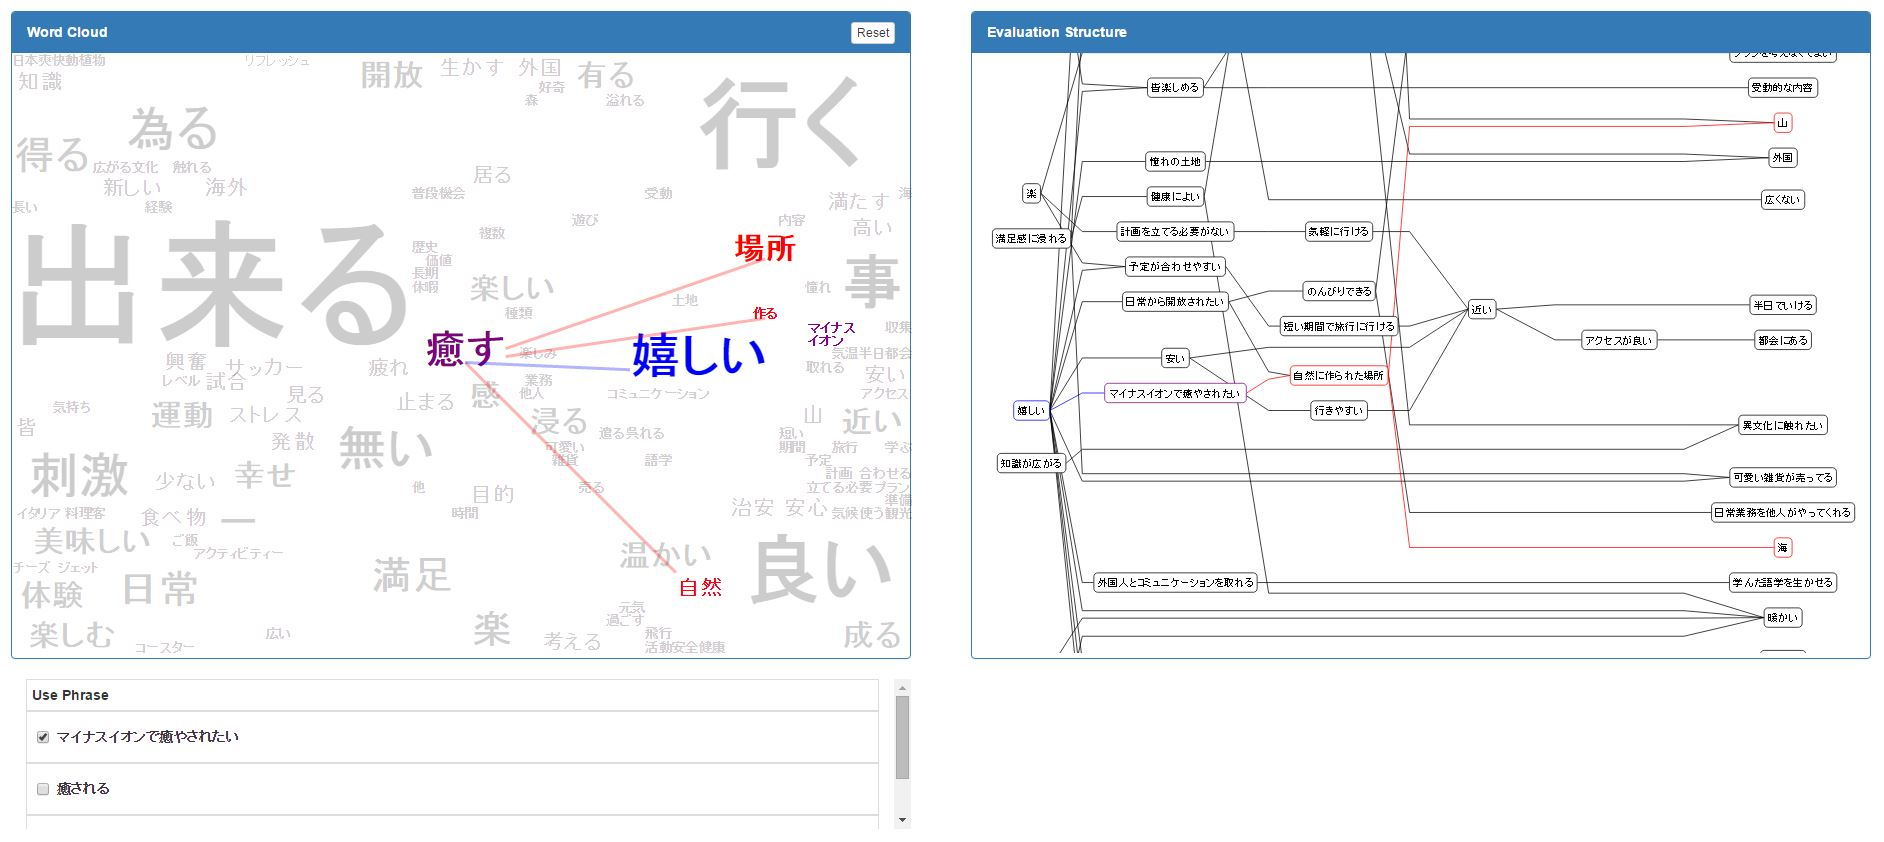
\includegraphics[width=\linewidth]{./png/cas2.JPG}
				}
			\end{center}
			\caption{注目評価項目の上位及び下位の評価項目探索}
	  		\label{fig:cas2}
		\end{figure}
			
%%考察
\chapter{考察}
	\section{比較実験}
	この節では比較実験についての考察を行う.
	タスク1の結果について,ネットワーク図ではノード数が増えるにつれタスク所要時間が増えていき,序論で取り上げた問題と同じ結果が起きた.
	その一方で,Nword Cloudでは,ノード数が増えてもタスク所要時間は大きく変動しなかった.
	また,正答率に関して,Nword Cloudとネットワーク図では有意差はなく,Nword Cloudが誤った情報を与える可視化手法ではないことがわかった.
	この結果から,Nword Cloudではネットワーク図の抱える問題を解決していると考えられる.
	
	タスク2の結果からは,評価構造内の位置関係を考慮してWord Cloud内の単語の座標を決定することの有効性を確かめることができた.
	Nword CloudとRword Cloud間のタスク所要時間の差の原因は,隣接する評価項目の単語が近くに配置されているためであると考えられる.
	また,ノード数が増えるにつれ,タスク所要時間の差が増加することから,大規模な評価構造分析の場合でもNword Cloudが有効であると考えられる.
	ネットワーク図ではタスク1とで様に,ノード数が増えるにつれタスク所要時間が増えていき,序論で取り上げた問題と同じ結果が起きた.
	しかし,ネットワーク図とNword Cloud間では所要時間での有意差は確認できなかった.
	Nword Cloudではノード数にかかわらず約半分の時間だったにも関わらず有意差が確認できなかった原因は,
	評価構造への習熟度に応じて所要時間が大きく異なったことが原因と考えられた.
	そこで,タスク2の所要時間から順位をつけ,ネットワーク図とNword Cloud間の順位の差でt検定を行ったところ,
	ノード数が136個の場合で有意差を確認することができた(図~\ref{fig:res10}).
	ここから,Nword Cloudではネットワーク図の抱える問題を解決していると考えられる.
	
	タスク3では,Nword Cloudはネットワーク図と比較し全てのノード数で2/3の所要時間であったが,ノード数が多い場合には有意差を確認することができなかった.
	また,Rword Cloudとネットワーク図でのタスク3所要時間にも有意差はなく,
	Word Cloudは頻出単語のフォントサイズが大きくなることから,多くの回答者が回答した項目を発見することに適していると想定していたが,そのような結果を得ることができなかった.
	
	\section{ケーススタディ}%%%尾上さん論文5.5.1が参考になるかも
	提案システムを3人の被験者に使用してもらい得た評価について考察する.
		\paragraph{有効性}
		有効性に関して4種類の観点から評価された.
		一つ目は評価構造の概観に関してである.
		ワードクラウドウィンドウは評価構造の概観に有効であり,評価構造内にどのような評価項目があるのか予想がつきやすくなった.
		二つ目は重要項目の発見に関してである.
		ワードクラウドウィンドウのフォントサイズによって評価構造の中で頻出する項目を発見でき,
		重要な項目の発見につながった.
		三つ目は評価項目間の関係性を把握に関してである.
		ワードクラウドウィンドウ内の注目単語をクリックすることで,クリックした単語と隣接する評価項目の単語を確認することができた.
		また,クリックした単語が使用されている評価項目が評価構造ウィンドウ内で強調されることで隣接する評価項目だけでなく,
		上位及び下位概念の項目を全て確認することができた.
		四つ目は評価項目のグループ分けである.
		ワードクラウドウィンドウでは評価構造内で隣接関係にある単語が近くに配置されているため,グループ分けを行うことができた.
		しかし,全ての単語がグループ分けできている訳ではなく,複数グループの評価項目に出現する単語などはグループ分けできなかった.
		
		\paragraph{操作性}
		操作性に関しては良い評価を得た.
		提案システムは,複数の操作ステップを必要とせず,また直感的な操作であったため,ユーザーは少しの説明と訓練で提案システムを使えるようになった.
		さらに,Webアプリケーションとして使用できるため,準備にかかる手間も少なく使いやすい.
		
		\paragraph{改善点}
		改善点について,評価項目と回答者の関係可視化についての意見を得た.
		ワードクラウドウィンドウで大きく表示されている単語は多くの回答者が注目している項目だと分かるものの,
		回答者数や回答者名の表示はなく,より詳細な分析を行うためには回答者の情報を表示することが必要である.
		二つ目は,連携についてである.
		ワードクラウドウィンドウで単語をクリックすることで,
		評価構造ウィンドウ内でクリックされた単語が使用されている評価項目をズームすることで
		より効率的な分析につながるという意見も得られた.
		
		以上,ケーススタディから得た評価の多くは肯定的であり,提案システムの有効性は確認できた.
		提案システムはシステム開発をする前に得たシステム要件を4つ満たしており目的を達成できていること言える.
		しかし,改善すべき点もあり今後の課題になる.
		
	\section{ユーザーフィードバック}
		\subsection{5段階評価アンケート結果}
		この項では,5段階評価アンケート結果についての考察を行う.
		多くの人が共有する評価項目の発見に関して,比較実験ではNword Cloudとネットワーク図では
		有意差が確認できなかったが,5段階評価アンケート結果では有意差を確認することができた.
		この結果から,Nword Cloudはネットワーク図の問題点である多くの人が回答する項目の発見に有効であることが確認できた.
		同時に,評価項目の関係性を同時に可視化している手法であることが確認できた.
		しかし,新しい発見や仮説構築につなげることへの有効性はネットワーク図と差は確認できなかった.
		この原因は,2つの可視化手法の可視化内容の違いだと考えられる.
		Nword Cloudでは,多くの人が共有する評価項目と評価項目の関係性を同時に可視化しているが,
		評価項目の関係性については詳細な情報を伝えることはできていない.
		Nword Cloudでは,注目する単語の評価項目と隣接する評価項目の詳細な文章や,
		より上位及び下位の評価項目の文章を確認することはできない.
		そこで,今後は隣接する評価項目の詳細な情報や,より上位及び下位の評価項目の情報を可視化する手法や,
		提案システムのようなネットワーク図とWord Cloud表示の同時表示するような機能が必要であると考えられる.
		
		\subsection{自由記述アンケート結果}
		この項では,自由記述アンケート結果に対する考察を行う.
		アンケートの結果は大きく2種類に分けることができた.
		一つ目は,提案手法であるWord Cloudの単語の配置計算についてである.
		単語の距離関係から単語間の関係性の予測が可能になり,その予測の確認を単語の文字色や線で行うことができる.
		このような単語の関係性を直感的に予測でき,その予測の正否の確認を即座に行える機能が有効であると確認できた.
		その一方で,提案手法によるWord Cloud可視化では,空白部分が目立ち単語の探索に悪影響をきたすことがあった.
		単語のフォントサイズを拡大することなどでの空白部分の削減は今後の課題とされる.
		また,単語を配置する際にフォントサイズが同じ複数の単語が横に並べられることで,
		単語間の切れ目を勘違いすることも確認された.単語間の距離感の設定も今後の課題とされる.
	
		二つ目は,インタラクションについてである.
		単語をクリックした際に発生する操作方法について,よりシンプルなデザインにすることや
		単語の探索機能,より分かりやすい関連語の表示など新しい機能を採用することで改善することが求められている.
		
		\begin{figure}
			\begin{center}
				\fbox{
				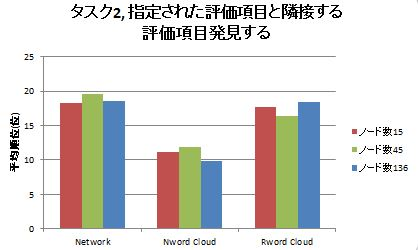
\includegraphics[width=\linewidth]{./png/res10.JPG}
				}
			\end{center}
			\caption{タスク2のタスク所要時間の平均順位}
	  		\label{fig:res10}
		\end{figure}

%%%結論と課題
\chapter{結論と今後の課題}
	\section{結論}
		本論文では,評価構造のノード数増加に伴う見やすさの低下,それによる評価構造分析の非効率化という問題に対して,
		評価項目内に出現する単語の頻度と,評価構造内での単語間の位置関係を反映した評価構造データ向けのテキストベースの可視化手法を提案し,
		同時に提案手法を用いた評価構造分析システムの開発を行った.
		評価実験によって確認した提案手法の有効性は次の3点である.
		
		はじめに,評価構造内の重要な評価項目の発見の効率化である.
		Nword Cloudとネットワーク図による比較実験では,評価構造内で頻出する単語を発見するタスクの所要時間が従来のネットワーク図よりも短く,
		5段階評価アンケートからも重要な評価項目の発見に関してネットワーク図よりも有効であることが確認できた.
		考察でも述べたように,提案手法では頻出する単語のフォントサイズを大きくし,また空白部分を出来るだけ減らしその分フォントサイズを大きく表示させた.
		これにより重要な単語,評価項目の発見を容易にした.
		
		次に,評価構造内での単語の関係性の可視化について述べる.
		3可視化手法による比較実験から,選択された単語と隣接する単語の発見するタスクの所要時間に関して,ネットワーク図よりも短く,
		Rword Cloudと比較しても短く,提案手法の有効性を確かめることができた.
		
		次に,評価構造の俯瞰表示の効率化に関して述べる.
		比較実験から,ノード数が増えた場合でも単語の発見の時間に変化はなかった.
		またケーススタディからも,評価構造の概観が可能であることが確認できた.
		
		最後に,ケーススタディから提案システムの有効性を確認することができた.
		提案手法によるWord Cloud表示とネットワーク図の連携,直感的で簡潔な操作などによって
		評価構造の概観から注目語の発見,注目語の詳細情報の確認,グループ分けなどに有効であることが示された.		
		%%これは,従来のネットワーク表示と比較し,エッジや助詞助動詞などの意味無し語を削減し,複数回出現する語を統合することによって,フォントサイズを大きく表示することができたのが
		
	\section{今後の課題}
		本論文で得られた結果を踏まえて,今後検討するべき課題を以下で述べる.
		提案手法に関しては5種類あげられる.
		
		一つ目は,単語の配置座標に関してである.
		提案手法による単語の配置座標計算では,隣接関係にある単語が近くに配置することを目的とし,その有効性を確かめることができた.
		今後はより多くの隣接語が近くに配置する計算手法が求められる.
		そのため,新しく制約条件を加えた計算や,力学モデルを考慮した座標計算などが考えられる.
		また,提案手法では単語間の距離が近すぎた場合に単語の切れ目が不明瞭な場合があるので,
		最適化計算を行う場合はこのようなことをなくすために制約条件を変更することも求められる.
		
		二つ目は,単語のフォントサイズに関してである.
		文字のサイズを大きくさせることは,評価構造の概観をより容易にするためには求められる.
		提案手法では,空白部分がまだ多く残っていたのでこれをさらに削減させ,その分フォントサイズを大きくすることが改善点の一つとしてあげられる.
		単語のフォントサイズについて,提案手法頻出語の線形比でフォントサイズを決定しているが,
		対数比などにすることで最小単語のフォントサイズを大きくすることも検証する必要がある.
		また,フォントサイズを出現頻度ではなく,tfidfなど他の値を用いることも考えられる.		
		
		三つ目は,より詳細な情報の可視化に関してである.
		ケーススタディで,Word Cloud内の注目単語の回答者人数や回答者名が分析には求められていることがわかった.
		このように,より多くの情報を可視化することがより効果的な分析には求められている.
		また,単語をマウスオーバーすることで,その単語が使用されている評価項目を表示する機能など,
		より簡単な操作で情報を表示する機能なども必要である.
		この他にも単語の検索機能や,品詞別で表示単語の絞り込み,副詞など提案手法では表示しなかった品詞の可視化,共起単語のより分かりやすい可視化などが
		効果的な分析に必要だと考えられる.
		
		四つ目は隣接関係の表示である.
		提案手法では,Word Cloud内の注目単語をクリックすることで隣接する単語の表示を行うが,
		より上位及び下位の評価項目の表示が求められていることがわかった.
		また,提案手法ではわからなかった注目単語と隣接する評価項目の文章の可視化も求められる.
		
		最後に,提案システムに関してはケーススタディからインタラクションについての改善が求められていることがわかった.
		現在の提案手法では,評価構造の持つ情報の一部を可視化出来ていないので,ネットワーク図など他の可視化結果と併置することが
		評価構造分析にとって必要である.
		そのため,よりシンプルなデザインやWord Cloudウィンドウのズーム機能,強調表示の改善などウィンドウごとの機能の向上と,
		機能間の連携をより向上させることが評価構造のより効果的な分析につながると考えられる.
		また,ネットワーク図と提案手法による可視化結果のモーフィングは2つの可視化結果の関係性を分かりやすく,
		効果的な分析につながると考えられる.

%======================================================================
%		謝辞
%======================================================================
\begin{acknowledgements}
	本研究では,小山田耕二教授から熱心な研究指導を賜りました.
	小山田教授からは,終始懇切丁寧なご指導,ご鞭撻を頂くとともに,研究遂行に当たり多岐にわたるご指摘を賜りました.
	神戸大学 システム情報学研究科の坂本尚久講師には,研究遂行にあたり数多くの適切なご教示を賜りました.
	京都大学学際融合教育研究推進センター政策のための科学ユニットの久木元伸如特定講師には,システム評価にあたり
	適切なご助言を賜りました.
	京都大学 工学研究科の尾上洋介博士には,評価グリッド法についての様々なご意見から
	システム開発やシステム評価に関するご助言など多岐にわたるご指摘を賜りました.
	また,これまで本研究を行うにあたって,ここに上げた以上に多くの方々のご協力がありました.
	ご協力いただいた皆様に熱く御礼申し上げます.
	最後に,家族をはじめとする私の学生生活を支えてくださったすべての皆様へ心から感謝の意を表します.
\end{acknowledgements}

%======================================================================
%		参考文献
%======================================================================
\bibliographystyle{kueethesis}
\bibliography{sotsuron}
\begin{thebibliography}{数字}
	\bibitem{sen1} 福田忠彦,福田亮子,人間工学ガイド: 感性を科学する方法,サイエンティスト社,175-176,(2009).
	\bibitem{egm6} J.Sanui,Visualization of users’requirements: Introduction of Evaluation Grid Method,Proceedings of the 3rd Design and Decision Support System in Architecture and Urban Planning Conference,365-374,(1996).
	\bibitem{egm7} 讃井純一郎,乾正雄,レパートリー・グリッド発展手法による住環境評価構造の抽出:認知心理学に基づく住環境評価に関する研究(1).日本建築学会計画系論文報告集,367,15-22,(1986).
	\bibitem{egm8} 尾上洋介,久木元伸如,小山田耕二, 可視化情報学会における会員満足度の因果関係分析, 可視化情報学会論文集,34,43-51,(2014).
	\bibitem{egm9} 本村陽一,金出武雄, ヒトの認知・評価構造の定量化モデリングと確率推論,電子情報通信学会技術研究報告,104,25-30,(2005).
	\bibitem{egm10} Y.Onoue,N.Kukimoto,M.Kioka,K.Koyamada,Visualizing Cognitive Structures Using a Layered Graph Drawing,In Proc of IEEE Pacific Visualization Poster,(2014).
	\bibitem{wc1} J.Steele,L.Noah,Beautiful visualization,O'Reilly Media Inc,40-60,(2010).
	\bibitem{rg1} G.A.Kelly,The Psychology of Personal Constructs,1 and 2,(1955).
	\bibitem{rd1} D.N.Hinkle,The change of personal constructs from the viewpoint of a theory of construct implications,PhD thesis,(1965).
	\bibitem{egm1} 高橋浩伸,大井尚行,インテリア空間における美的価値観と評価構造: 現代日本人の建築空間における美意識に関する基礎的研究,日本建築学会環境系論文集,615,59-64,(2007).
	
	\bibitem{egm2} 讃井純一郎,商品企画のためのインタビュー調査: 従来型インタビュー調査と評価グリッド法の現状と課題 (< 特集> 品質経営のための調査の方法),品質,33,13-20,(2003).
	\bibitem{egm11} Y.Tsuchida,Y.Kozaka,Development and application of a supporting tool for the evaluation grid method,Architectural Institute of Japan Journal of Technology and Design,14,27,205-208,(2008).
	\bibitem{egm12} S.Nagasawa,Revision and verification of ”seven tools for new product planning”,KANSEI Engineering International,3,4,3-8,(2002).
	\bibitem{net1} Y.Onoue,N.Kukimoto,N.Sakamoto,K.Koyamada,Network Coarse-Graining for Evaluation Structures,In Proc of International Conference on Simulation Technology,34,447-450,(2015).
	\bibitem{kh3} C.E.Osgood,G.J.Suci,P.H.Tennenbaum,The measurement of Meaning,University of Illinois Press,(1957).
	\bibitem{kh1} 樋口耕一,テキスト型データの計量的分析,理論と方法,数理社会学会,19,101-115,(2004).
	\bibitem{kh2} 樋口耕一,社会調査のための計量テキスト分析 ―内容分析の継承と発展を目指して―,ナカニシヤ出版,(2004).
	\bibitem{wt1} M.Wattenberg,B.V.Fernanda,The Word Tree,an interactive visual concordance,IEEE Transactions on Visualization and Computer Graphic,14,1221-1228,(2008).
	\bibitem{wg1} P.Riehmann,H.Gruendl,M.Potthast,M.Trenkmann,B.Stein,B.Froehlich,WORDGRAPH: Keyword-in-Context Visualization for NETSPEAK's Wildcard Search,IEEE Transactions on Visualization and Computer Graphics,18.9,1411-1423,(2012).
	\bibitem{wc2} F.B.Viégas,M.Wattenberg,J.Feinberg,Participatory visualization with Wordle,IEEE Transactions on Visualization and Computer Graphics,15,6,1137–44,(2009).

	\bibitem{or1} E.G.Nieto,F.S.Roman,P.Pagliosa,W.Casaca,E.S.Helou,M.C.Oliveira,L.G.Nonato,Similarity Preserving Snippet-Based Visualization of Web Search Results,IEEE Transactions on Visualization and Computer Graphics,20,457-470,(2014).
	%\bibitem{pn1} F.V.Ham,M.Wattenberg,B.V.Fernanda,Mapping text with phrase nets,IEEE transactions on visualization and computer graphics,15,1169-1176,(2009).
	%\bibitem{jig1} C.Gorg,J.Stasko,Combining Computational Analyses and Interactive Visualization for Document Exploration and Sensemaking in Jigsaw,IEEE Transactions on Visualization and Computer Graphics,19,1646-1663,(2013).
	\bibitem{fta2} I.Ada,K.Thiel,M.R.Berthold,Distance aware tag clouds,IEEE International Conference on Systems,2316–2322,(2010).
	\bibitem{fta1} X.Huang,W.Lai,Force-transfer: a new approach to removing overlapping nodes in graph layout,Proceedings of the 26th Australasian computer science conference,16,349-358,(2003).
	\bibitem{or2} E.G.Nieto,W.Casaca,D.Motta,I.Hartmann,G.Taubin,L.Nonato,Dealing with Multiple Requirements in Geometric Arrangements,IEEE Transactions on Visualization and Computer Graphics,1,(2015).
	\bibitem{fsa1} E.Peter,W.Lai,Algorithms for disjoint node images,Key Centre for Software Technology,(1991).
	\bibitem{rwc1} H.Strobelt,M.Spicker,A.Stoffel,D.Keim,O.Deussen,Rolled‐out Wordles: A Heuristic Method for Overlap Removal of 2D Data Representatives,Computer Graphics Forum,31,1135-1144,(2012).
	\bibitem{int1} Cormen,H.Thomas,Introduction to algorithms,MIT press,(2009).
	\bibitem{mcb1} T.Kuo,K.Yamamoto,Y.Matsumoto,Applying Conditional Random Fields to Japanese Morphological Analysis,Proceedings of the 2004 conference on empirical methods in natural language processing,230-237,(2004).
	\bibitem{hak1} 尾上洋介,因果グラフのビジュアル分析に関する研究—評価グリッド法における評価構造分析を通じて—,博士論文,(2016).
	%\bibitem{egm3} 来田宣幸,赤井聡文,野球における球速と球速感の関係,日本認知心理学会発表論文集,42,(2009).
	%\bibitem{egm4} 中前光弘,順位法を用いた視覚評価の信頼性について: 順序尺度の解析と正規化順位法による尺度構成法.日放技学誌,56,725-730,(2000).
\end{thebibliography}

%======================================================================
%		付録
%======================================================================
\appendix


\end{document}
% Local Variables:
% fill-column: 70
% End:
